\documentclass{beamer}
\usepackage{xcolor}
% \usetheme{Marburg}
\usecolortheme{orchid}
\usepackage{pifont}
\usepackage{nicefrac}
\usepackage{csquotes}
\usepackage{changepage}
\usepackage{cancel} 
\makeatletter
\def\blfootnote{\gdef\@thefnmark{}\@footnotetext}
\makeatother
\newcommand{\crossout}[2][red]{%
  \begin{tikzpicture}[baseline=(texte.base)]
    % Nœud pour le texte
    \node[inner sep=0pt, outer sep=0pt] (texte) {#2};
    % Dessiner la croix (deux lignes diagonales)
    \draw[overlay, #1, line width=0.5pt] 
      (texte.north west) -- (texte.south east); % Ligne diagonale 1
    \draw[overlay, #1, line width=0.5pt] 
      (texte.north east) -- (texte.south west); % Ligne diagonale 2
  \end{tikzpicture}%
}
\usepackage[  
backend=biber,
style=alphabetic,
]{biblatex}
\addbibresource{gcm.bib}
\usepackage{hyperref, xcolor, cmbright,diagbox,colortbl,tikz,graphicx,algorithm2e,cancel,verbatim, graphicx,
listings,float,amsmath,amssymb,array,subfiles,bussproofs,
rotating,MnSymbol,hyperref,mathtools,subcaption,caption}
\newtheorem{proposition}{Proposition}
\usetikzlibrary{overlay-beamer-styles}
\usetikzlibrary{automata, positioning,graphs,shapes, arrows, calc}

\newcommand{\set}[1]{\{#1\}}
\newcommand{\vertex}[2]{%
  \begin{tikzpicture}[baseline=-1ex]%
    \node [rectangle,rounded corners=2mm,inner sep=0.5mm,fill=#2] {$#1$};%
  \end{tikzpicture}%
}
\newcommand{\graphbox}[8]{
  \begin{scope}[xshift=#2,yshift=#3]
    \draw [rounded corners=2mm] (0,0) rectangle (#4,-#5);
    \node at (0,0mm) [anchor=north west,inner sep=1mm] {#1};
    \begin{scope}[xshift=#4/2+#6,yshift=#7] 
    #8
    \end{scope}
  \end{scope}
}

\newcommand{\opn}[1]{\operatorname{#1}}

\graphicspath{ {.} }

\title{Termination of Graph Rewriting
using Weighted Type Graphs
over Non-well-founded Semirings}
\setbeamertemplate{footline}[frame number]


\usetheme{default}% base theme

% default appearance
% \setbeamercolor{structure}{fg=blue}

% % code run at the start of each \section
% \AtBeginSection[]{
%   % a simple section title slide
%   \begin{frame}[plain]
%     \centering\Huge\insertsection
%   \end{frame}

%   % change appearance depending on section number
%   \ifcase\value{section} % 0 (no section) -> fallthrough to default
%   \or % section 1
%     \setbeamercolor{structure}{fg=blue}
%     \usebackgroundtemplate{} % clear background
%     \setcounter{framenumber}{0}%
%   \or % section 2
%     \setbeamercolor{structure}{fg=teal}
%     \usebackgroundtemplate{\includegraphics[width=\paperwidth,height=\paperheight]{bg-section2.pdf}}
%     \setcounter{framenumber}{0}%
%   \or % section 3
%     \setbeamercolor{structure}{fg=violet}
%     \usebackgroundtemplate{\tikz[overlay,remember picture] \fill[black!10] (current page.south west) rectangle (current page.north east);}
%     \setcounter{framenumber}{0}%
%   \else
%     % fallback for later sections
%     \setbeamercolor{structure}{fg=black}
%     \usebackgroundtemplate{}
%   \fi
% }

\begin{document}
% \date{\today}
\date{}
\author{Qi QIU}
\institute[VFU] % (optional)
{
	Supervisor: Xavier URBAIN\\
	Université Claude Bernard Lyon 1, France \\
  Université de Lorraine, France\\
}

\maketitle
 
\begin{frame}{Plan (for myself)}
  \begin{itemize}
    \item Introduction  
          \begin{itemize}
            \item Graphs and Graph Morphisms
            \item Double Pushout Diagram (DPO)
            \item Graph rewriting using DPO 
                  \begin{itemize}
                    \item Example of DPO graph rewriting : grsaa
                  \end{itemize}
            \item Termination of DPO graph rewriting systems
                  \begin{itemize}
                    \item Example: looping and terminating examples
                  \end{itemize}
          \end{itemize}
    \item Type graph method in theory 
    \item Type graph method in practice and the introduction of the main problem
    \item Morphism weight (by a example)
    \item Graph weight (by a example)
    \item A condition that weighted type graphs must satisfy
    \item Rule $\varphi$
    \item Example with rule $\varphi$
    \item Sufficient condition for termination using weighted type graph
    \item Sufficient condition simplified
    \item Example
    \item Example : termination of rule $\varphi$
    \item How to find a weighted type graph in practice
    \item Experimental results
    \item Acknowledgements
    \item Conclusion
  \end{itemize}
\end{frame}
\begin{frame}{Outline}
  \tableofcontents[hideallsubsections]
\end{frame} 
\section{Introduction}
\begin{frame}
  \tableofcontents
\end{frame}

\subsection{Graphs and Graph Morphisms}
\begin{frame}{Graphs}
\begin{adjustwidth}{-0.5cm}{0cm}
Graphs are \textcolor{red}{finite} and \textcolor{blue}{directed} with:
  \begin{itemize}
      \item Parallel edges,
      \item Labeled edges,
      \item Finite labels.
  \end{itemize}
      Example:
      \begin{itemize}
        \item Graph $G$ with 3 nodes. 
        \item 2 edges from node 1 to node 2 labeled by $a$.
        \item 1 edge from node 2 to node 3 labeled by $b$.
      \end{itemize}
      Notation:
        \begin{center} 
          \resizebox{0.5\textwidth}{!}{
          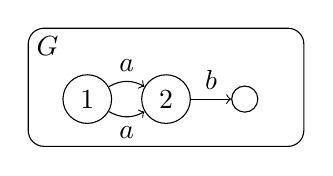
\begin{tikzpicture}
              \graphbox{\(G\)}{00mm}{-20mm}{35mm}{15mm}{2mm}{-5mm}{ 
                  \coordinate (o) at (-2mm,-4mm); 
                  \node[draw,circle] (l1) at ($(o)+(-10mm,0mm)$) {1};
                  \node[draw,circle] (l3) at ($(l1)+(1,0)$) {2};
                  \node[draw,circle] (l4) at ($(l1)+(2,0)$) {};
                  \draw[->] (l1) edge[bend right]  node[midway,below] {$a$} (l3);
                  \draw[->] (l1) edge[bend left] node[midway,above] {$a$}  (l3);
                  \draw[->] (l3) -- (l4) node[midway,above] {$b$};
                  % \draw[->] (l4) -- (l2) node[midway,above] {$a$};
              }   
          \end{tikzpicture} 
      }
      \end{center}
      \begin{itemize}
            \item \alert{Graphs} are contained \alert{in boxes}
            \item \alert{Graph name} $G$ is placed in the \alert{top left corner}
            \item Numbers in nodes are \alert{identifiers}, ommitted when not relevant
      \end{itemize}
\end{adjustwidth}
\end{frame} 


\begin{frame}{Inclusion (morphism)}
  Morphisms: structure-preserving functions between graphs

  Isomorphisms: bijective morphisms

  \textbf{Inclusions}: morphisms that are indentity functions
  
  Example in a viasual notion:
          \begin{center} 
            \resizebox{0.9\textwidth}{!}{
                \begin{tikzpicture}
                    \graphbox{$L$}{39mm}{0mm}{35mm}{35mm}{2mm}{-5mm}{
                        \coordinate (delta) at (0,-18mm);
                        \node[draw,circle,red] (l1) at ($(delta)+(-1,1.5)$) {1};
                        \node[draw,circle,red] (l2) at ($(delta)+(1,1.5)$) {2};
                        \node[draw,circle,red] (l3) at ($(delta)+(0,0)$) {3};
                        \draw[->,red] (l1) -- (l3) node[midway,left] {$s$};
                        \draw[->,red] (l2) -- (l3) node[midway,right] {$s$};
                        \draw[->,red] (l3) edge [loop below] node {0} (l3);
                    }
                        \node () at (77mm,-18mm) {$\overset{h}{\rightarrowtail}$};
                    \graphbox{$R$}{80mm}{0mm}{50mm}{35mm}{2mm}{-5mm}{
                        \coordinate (delta) at (-10mm,-18mm);
                        \node[draw,circle,red] (r1) at ($(delta)+(-1,1.5)$) {1};
                        \node[draw,circle,red] (r2) at ($(delta)+(0.5,1.5)$) {2};
                        \node[draw,circle,red] (r3) at ($(delta)+(0,0)$) {3};
                        \node[draw,circle] (r4) at ($(delta)+(1,0)$) {};
                        \node[draw,circle] (r5) at ($(r2)+(1.5,0)$) {};
                        \draw[->] (r1) edge[bend right] node[midway,left] {$s$} (r3) ; 
                        \draw[->] (r2) -- (r4) node[midway,right] {$s$};
                        \draw[->] (r4) edge [loop below] node {0} (r4);
                        \draw[->] (r5) edge [loop below] node {0} (r5);
                        \draw[->] (r5) edge [loop right] node {0} (r5);
                        \draw[->] (r5) edge [loop left] node {0} (r5);
                        \draw[->,red] (r1) edge node[midway,left] {$s$} (r3) ;
                        \draw[->,red] (r2) edge node[midway,right] {$s$} (r3) ; 
                        \draw[->,red] (r3) edge [loop below] node {0} (r3); 
                    }
                \end{tikzpicture}
                }
        \end{center}
        \begin{itemize}
            % \item \alert{Graphs} are contained \alert{in boxes}
            % \item \alert{Graph name} is placed in the \alert{top left corner}
            % \item \alert{Domain} is represented as a \alert{subgraph of codomain}
            % \item \alert{Corresponding elements} have the \alert{same position}
            \item \textcolor{red}{$\overset{h}{\rightarrowtail}$ between the boxes} marques an inclusion named $h$.
            % \item nodes $v$ and $h(v)$ marked by the same natural number
            % \item edges $e$ and $h(e)$ have the same spatial position
        \end{itemize}
        %  \begin{itemize}
        %     \item nodes of domain $L$ are assigned natural numbers 
        %     \item nodes of codomain $R$ are assigned natural numbers of their corresponding nodes in $L$
        %     \item s
        %  \end{itemize}
    % Inclusion : morphism $h: L \rightarrowtail R$ with $L \mathop{\subseteq} R$.
\end{frame}

\begin{frame}{Graph rewriting rule}
  \textbf{Rules} $\varphi \mathop{=} (L \overset{l}{\leftarrowtail} K \overset{r}{\rightarrowtail} R)$ consist of inclusions $l$ and $r$. 
   \begin{itemize}
       \item Running example $\varphi$:
        % \begin{center} 
    \resizebox{0.9\textwidth}{!}{
    \begin{tikzpicture}
        \graphbox{\( L \)}{0mm}{-3mm}{34mm}{12mm}{2mm}{2mm}{
            \coordinate (o) at (0mm,-8mm); 
            \node[draw,circle] (l1) at ($(o)+(-10mm,0mm)$) {1};
            \node[draw,circle] (l2) at ($(l1)+(2,0)$) {2};
            \node[draw,circle] (l3) at ($(l1)+(1,0)$) {3};
            \draw[->] (l1) -- (l3) node[midway,above] {$a$};
            \draw[->] (l3) -- (l2) node[midway,above] {$a$};
        } 

        \graphbox{\( K \)}{40mm}{-3mm}{34mm}{12mm}{2mm}{2mm}{
            \coordinate (o) at (0mm,-8mm); 
            \node[draw,circle] (l1) at ($(o)+(-10mm,0mm)$) {1};
            \node[draw,circle] (l2) at ($(l1)+(2,0)$) {2};
        }  

        \graphbox{\( R \)}{80mm}{-3mm}{45mm}{12mm}{2mm}{2mm}{
            \coordinate (o) at (-5mm,-8mm); 
            \node[draw,circle] (l1) at ($(o)+(-10mm,0mm)$) {1};
            \node[draw,circle] (l2) at ($(l1)+(3,0)$) {2};
            \node[draw,circle] (l3) at ($(l1)+(1,0)$) {4};
            \node[draw,circle] (l4) at ($(l1)+(2,0)$) {5};
            \draw[->] (l1) -- (l3) node[midway,above] {$a$};
            \draw[->] (l3) -- (l4) node[midway,above] {$b$};
            \draw[->] (l4) -- (l2) node[midway,above] {$a$};
        }    
        \node () at (37mm,-8mm) {\( \overset{l}{\leftarrowtail} \)}; % K -> L
        \node () at (77mm,-8mm) {\( \overset{r}{\rightarrowtail} \)}; % K -> R
    \end{tikzpicture}
    }         
        % \end{center}
   \end{itemize} 
    Rule $\varphi' \mathop{=} (L' \overset{l'}{\leftarrowtail} K' \overset{r'}{\rightarrowtail} R')$ and $\varphi$ are \alert{equivalent} if there are \alert{isomorphisms $a,b,c$} such that $a \circ l' = l \circ b$ and $c \circ r' = r \circ b$:
            \begin{center}
                    \resizebox{0.40\textwidth}{!}{
                        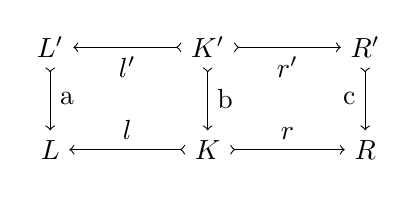
\begin{tikzpicture}
                                \node (I) at (0,-0.7) {$K'$};
                                \node (L) at (-2,-0.7) {$L'$};
                                \node (R) at (2,-0.7) {$R'$};
                                \node (G) at (-2,-2) {$L$};
                                \node (C) at (0,-2) {$K$};
                                \node (H) at (2,-2) {$R$};
                                \draw [>->] (I) to  node [midway,below] {$l'$} (L);
                                \draw [>->] (I) to  node [midway,below] {$r'$} (R);
                                \draw [>->] (L) to node [midway,right] {\alert{a}} (G);
                                \draw [>->] (I) to node [midway,right] {\alert{b}} (C);
                                \draw [>->] (R) to node [midway,left] {\alert{c}} (H);
                                \draw [>->] (C) to node [midway,above] {$l$} (G);
                                \draw [>->] (C) to node [midway,above] {$r$} (H);
                                \node [at=($(I)!.5!(G)$)] { };
                                \node [at=($(I)!.5!(H)$)] { };
                            \end{tikzpicture}
                    }
                \end{center}
A rule equivalent to $\varphi$:
     \resizebox{0.9\textwidth}{!}{
           \begin{tikzpicture}
                \graphbox{\( L' \)}{0mm}{-3mm}{34mm}{12mm}{2mm}{2mm}{
                    \coordinate (o) at (0mm,-8mm); 
                    \node[draw,circle] (l1) at ($(o)+(-10mm,0mm)$) {6};
                    \node[draw,circle] (l2) at ($(l1)+(2,0)$) {8};
                    \node[draw,circle] (l3) at ($(l1)+(1,0)$) {7};
                    \draw[->] (l1) -- (l3) node[midway,above] {$a$};
                    \draw[->] (l3) -- (l2) node[midway,above] {$a$};
                } 
        
                \graphbox{\( K' \)}{40mm}{-3mm}{34mm}{12mm}{2mm}{2mm}{
                    \coordinate (o) at (0mm,-8mm); 
                    \node[draw,circle] (l1) at ($(o)+(-10mm,0mm)$) {6};
                    \node[draw,circle] (l2) at ($(l1)+(2,0)$) {7};
                }  
        
                \graphbox{\( R' \)}{80mm}{-3mm}{45mm}{12mm}{2mm}{2mm}{
                    \coordinate (o) at (-5mm,-8mm); 
                    \node[draw,circle] (l1) at ($(o)+(-10mm,0mm)$) {6};
                    \node[draw,circle] (l2) at ($(l1)+(3,0)$) {7};
                    \node[draw,circle] (l3) at ($(l1)+(1,0)$) {9};
                    \node[draw,circle] (l4) at ($(l1)+(2,0)$) {10};
                    \draw[->] (l1) -- (l3) node[midway,above] {$a$};
                    \draw[->] (l3) -- (l4) node[midway,above] {$b$};
                    \draw[->] (l4) -- (l2) node[midway,above] {$a$};
                }    
                \node () at (37mm,-8mm) {\( \overset{l}{\leftarrowtail} \)};  
                \node () at (77mm,-8mm) {\( \overset{r}{\rightarrowtail} \)}; %
            \end{tikzpicture}
            }         
\end{frame}

\begin{frame}{Graph Rewriting}
 
 Rewriting steps $G \mathop{\Rightarrow}_\varphi H$ using rule $\varphi$ are commutative diagrams with an equivalent rule $L' \overset{l'}{\leftarrowtail} K' \overset{r'}{\rightarrowtail} R'$ where all morphisms are inclusions:
         \begin{center}
          \resizebox{0.40\textwidth}{!}{
              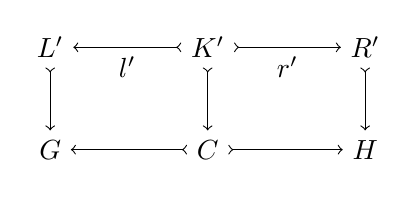
\begin{tikzpicture}
                    \node (I) at (0,-0.7) {$K'$};
                    \node (L) at (-2,-0.7) {$L'$};
                    \node (R) at (2,-0.7) {$R'$};
                    \node (G) at (-2,-2) {$G$};
                    \node (C) at (0,-2) {$C$};
                    \node (H) at (2,-2) {$H$};
                    \draw [>->] (I) to  node [midway,below] {$l'$} (L);
                    \draw [>->] (I) to  node [midway,below] {$r'$} (R);
                    \draw [>->] (L) to node [midway,left] {} (G);
                    \draw [>->] (I) to node [midway,right] { } (C);
                    \draw [>->] (R) to node [midway,left] { } (H);
                    \draw [>->] (C) to node [midway,above] { } (G);
                    \draw [>->] (C) to node [midway,above] { } (H);
                    \node [at=($(I)!.5!(G)$)] {} ;
                    \node [at=($(I)!.5!(H)$)] {};
                  \end{tikzpicture}
          }
      \end{center}
      % such that all 
      % \begin{itemize}
      %   % \item $L' \overset{l'}{\leftarrowtail} K' \overset{r'}{\rightarrowtail} R'$ is equivalent to $\varphi$,
      %   \item 
      %   % \item $G = L' \cup C$,
      %   % \item $H = R' \cup C$.
      % \end{itemize}

      A rewriting step using $\varphi$:
  \begin{center}
    \resizebox{0.7\textwidth}{!}{
      \begin{tikzpicture}
              \graphbox{\( L\)}{0mm}{5mm}{34mm}{20mm}{2mm}{-5mm}{
                  \coordinate (o) at (0mm,-8mm); 
                  \node[draw,circle] (l1) at ($(o)+(-10mm,0mm)$) {1};
                  \node[draw,circle] (l2) at ($(l1)+(2,0)$) {2};
                  \node[orange,draw,circle] (l3) at ($(l1)+(1,0)$) {3};
                  \draw[orange,->] (l1) -- (l3) node[midway,above] {$a$};
                  \draw[orange,->] (l3) -- (l2) node[midway,above] {$a$};
              } 

              \graphbox{\( K \)}{40mm}{5mm}{34mm}{20mm}{2mm}{-5mm}{
                  \coordinate (o) at (0mm,-8mm); 
                  \node[draw,circle] (l1) at ($(o)+(-10mm,0mm)$) {1};
                  \node[draw,circle] (l2) at ($(l1)+(2,0)$) {2};
              }  

              \graphbox{\( R \)}{80mm}{5mm}{45mm}{20mm}{2mm}{-5mm}{
                  \coordinate (o) at (-5mm,-8mm); 
                  \node[draw,circle] (l1) at ($(o)+(-10mm,0mm)$) {1};
                  \node[draw,circle] (l2) at ($(l1)+(3,0)$) {2};
                  \node[red,draw,circle] (l3) at ($(l1)+(1,0)$) {4};
                  \node[red,draw,circle] (l4) at ($(l1)+(2,0)$) {5};
                  \draw[red,->] (l1) -- (l3) node[midway,above] {$a$};
                  \draw[red,->] (l3) -- (l4) node[midway,above] {$b$};
                  \draw[red,->] (l4) -- (l2) node[midway,above] {$a$};
              }    

              \graphbox{\( G  \)}{0mm}{-22mm}{34mm}{30mm}{2mm}{-10mm}{
                  \coordinate (o) at (0mm,-3mm); 
                  \node[draw,circle] (l1) at ($(o)+(-10mm,0mm)$) {1};
                  \node[draw,circle] (l2) at ($(l1)+(2,0)$) {2};
                  \node[draw,circle,orange] (l3) at ($(l1)+(1,0)$) {3};
                  \node[blue, draw,circle] (l4) at ($(l2)+(0,-1)$) {6};
                  \draw[orange,->] (l1) -- (l3) node[midway,above] {$a$};
                  \draw[orange,->] (l3) -- (l2) node[midway,above] {$a$};
                  \draw[blue,->] (l2) -- (l4) node[midway,right] {$a$};
                %   \node[blue,draw,circle] (l6) at ($(l1)+(0,-1)$) {7};
                %   \draw[blue,<-] (l1) -- (l6) node[midway,left] {$a$};
              }    

              \graphbox{\( C  \)}{40mm}{-22mm}{34mm}{30mm}{2mm}{-10mm}{
                  \coordinate (o) at (0mm,-3mm); 
                  \node[draw,circle] (l1) at ($(o)+(-10mm,0mm)$) {1};
                  \node[draw,circle] (l2) at ($(l1)+(2,0)$) {2};
                  \node[blue,draw,circle] (l4) at ($(l2)+(0,-1)$) {6};
                  \draw[blue,->] (l2) -- (l4) node[midway,right] {$a$};
                %   \node[blue,draw,circle] (l6) at ($(l1)+(0,-1)$) {7};
                %   \draw[blue,<-] (l1) -- (l6) node[midway,left] {$a$};
              }    

              \graphbox{\( H   \)}{80mm}{-22mm}{45mm}{30mm}{2mm}{-10mm}{
                  \coordinate (o) at (-5mm,-3mm); 
                  \node[draw,circle] (l1) at ($(o)+(-10mm,0mm)$) {1};
                  \node[draw,circle] (l2) at ($(l1)+(3,0)$) {2};
                  \node[draw,circle,red] (l3) at ($(l1)+(1,0)$) {4};
                  \node[draw,circle,red] (l4) at ($(l1)+(2,0)$) {5};
                  \node[blue,draw,circle] (l5) at ($(l2)+(0,-1)$) {6};
                %   \node[blue,draw,circle] (l6) at ($(l1)+(0,-1)$) {7};
                %   \draw[blue,<-] (l1) -- (l6) node[midway,left] {$a$};
                  \draw[red,->] (l1) -- (l3) node[midway,above] {$a$};
                  \draw[red,->] (l3) -- (l4) node[midway,above] {$b$};
                  \draw[red,->] (l4) -- (l2) node[midway,above] {$a$};
                  \draw[blue,->] (l2) -- (l5) node[midway,right] {$a$};
              }    

              \node () at (37mm,-8mm) {\( \overset{l}{\leftarrowtail} \)}; % K -> L
              \node () at (77mm,-8mm) {\( \overset{r}{\rightarrowtail} \)}; % K -> R
              \node () at (17mm,-18mm) {\( \downarrowtail \)};
              \node () at (37mm,-33mm) {\( \leftarrowtail \)};
              \node () at (52mm,-18mm) {\( \downarrowtail \)};
              \node () at (92mm,-18mm) {\( \downarrowtail \)};
              \node () at (77mm,-33mm) {\( \rightarrowtail \)}; % C -> H
      \end{tikzpicture}
      }
   \end{center}
\end{frame} 

\begin{frame}{A rewriting step of the running rule (to do : delete)}
  Rewriting rule $\varphi$:
  \begin{center}
    \resizebox{0.8\textwidth}{!}{
      \begin{tikzpicture}
              \graphbox{\( L\)}{0mm}{5mm}{34mm}{20mm}{2mm}{-5mm}{
                  \coordinate (o) at (0mm,-8mm); 
                  \node[draw,circle] (l1) at ($(o)+(-10mm,0mm)$) {1};
                  \node[draw,circle] (l2) at ($(l1)+(2,0)$) {2};
                  \node[orange,draw,circle] (l3) at ($(l1)+(1,0)$) {3};
                  \draw[orange,->] (l1) -- (l3) node[midway,above] {$a$};
                  \draw[orange,->] (l3) -- (l2) node[midway,above] {$a$};
              } 

              \graphbox{\( K \)}{40mm}{5mm}{34mm}{20mm}{2mm}{-5mm}{
                  \coordinate (o) at (0mm,-8mm); 
                  \node[draw,circle] (l1) at ($(o)+(-10mm,0mm)$) {1};
                  \node[draw,circle] (l2) at ($(l1)+(2,0)$) {2};
              }  

              \graphbox{\( R \)}{80mm}{5mm}{45mm}{20mm}{2mm}{-5mm}{
                  \coordinate (o) at (-5mm,-8mm); 
                  \node[draw,circle] (l1) at ($(o)+(-10mm,0mm)$) {1};
                  \node[draw,circle] (l2) at ($(l1)+(3,0)$) {2};
                  \node[red,draw,circle] (l3) at ($(l1)+(1,0)$) {4};
                  \node[red,draw,circle] (l4) at ($(l1)+(2,0)$) {5};
                  \draw[red,->] (l1) -- (l3) node[midway,above] {$a$};
                  \draw[red,->] (l3) -- (l4) node[midway,above] {$b$};
                  \draw[red,->] (l4) -- (l2) node[midway,above] {$a$};
              }    
              \node () at (37mm,-8mm) {\( \overset{l}{\leftarrowtail} \)}; % K -> L
              \node () at (77mm,-8mm) {\( \overset{r}{\rightarrowtail} \)}; % K -> R
      \end{tikzpicture}
      }
   \end{center}
  
   A rewriting step $G \Rightarrow_\varphi H$:
  \begin{center}
    \resizebox{0.8\textwidth}{!}{
      \begin{tikzpicture}
              \graphbox{\( L\)}{0mm}{5mm}{34mm}{20mm}{2mm}{-5mm}{
                  \coordinate (o) at (0mm,-8mm); 
                  \node[draw,circle] (l1) at ($(o)+(-10mm,0mm)$) {1};
                  \node[draw,circle] (l2) at ($(l1)+(2,0)$) {2};
                  \node[orange,draw,circle] (l3) at ($(l1)+(1,0)$) {3};
                  \draw[orange,->] (l1) -- (l3) node[midway,above] {$a$};
                  \draw[orange,->] (l3) -- (l2) node[midway,above] {$a$};
              } 

              \graphbox{\( K \)}{40mm}{5mm}{34mm}{20mm}{2mm}{-5mm}{
                  \coordinate (o) at (0mm,-8mm); 
                  \node[draw,circle] (l1) at ($(o)+(-10mm,0mm)$) {1};
                  \node[draw,circle] (l2) at ($(l1)+(2,0)$) {2};
              }  

              \graphbox{\( R \)}{80mm}{5mm}{45mm}{20mm}{2mm}{-5mm}{
                  \coordinate (o) at (-5mm,-8mm); 
                  \node[draw,circle] (l1) at ($(o)+(-10mm,0mm)$) {1};
                  \node[draw,circle] (l2) at ($(l1)+(3,0)$) {2};
                  \node[red,draw,circle] (l3) at ($(l1)+(1,0)$) {4};
                  \node[red,draw,circle] (l4) at ($(l1)+(2,0)$) {5};
                  \draw[red,->] (l1) -- (l3) node[midway,above] {$a$};
                  \draw[red,->] (l3) -- (l4) node[midway,above] {$b$};
                  \draw[red,->] (l4) -- (l2) node[midway,above] {$a$};
              }    

              \graphbox{\( G  \)}{0mm}{-22mm}{34mm}{30mm}{2mm}{-10mm}{
                  \coordinate (o) at (0mm,-3mm); 
                  \node[draw,circle] (l1) at ($(o)+(-10mm,0mm)$) {1};
                  \node[draw,circle] (l2) at ($(l1)+(2,0)$) {2};
                  \node[draw,circle,orange] (l3) at ($(l1)+(1,0)$) {3};
                  \node[blue, draw,circle] (l4) at ($(l2)+(0,-1)$) {6};
                  \draw[orange,->] (l1) -- (l3) node[midway,above] {$a$};
                  \draw[orange,->] (l3) -- (l2) node[midway,above] {$a$};
                  \draw[blue,->] (l2) -- (l4) node[midway,right] {$a$};
                %   \node[blue,draw,circle] (l6) at ($(l1)+(0,-1)$) {7};
                %   \draw[blue,<-] (l1) -- (l6) node[midway,left] {$a$};
              }    

              \graphbox{\( C  \)}{40mm}{-22mm}{34mm}{30mm}{2mm}{-10mm}{
                  \coordinate (o) at (0mm,-3mm); 
                  \node[draw,circle] (l1) at ($(o)+(-10mm,0mm)$) {1};
                  \node[draw,circle] (l2) at ($(l1)+(2,0)$) {2};
                  \node[blue,draw,circle] (l4) at ($(l2)+(0,-1)$) {6};
                  \draw[blue,->] (l2) -- (l4) node[midway,right] {$a$};
                %   \node[blue,draw,circle] (l6) at ($(l1)+(0,-1)$) {7};
                %   \draw[blue,<-] (l1) -- (l6) node[midway,left] {$a$};
              }    

              \graphbox{\( H   \)}{80mm}{-22mm}{45mm}{30mm}{2mm}{-10mm}{
                  \coordinate (o) at (-5mm,-3mm); 
                  \node[draw,circle] (l1) at ($(o)+(-10mm,0mm)$) {1};
                  \node[draw,circle] (l2) at ($(l1)+(3,0)$) {2};
                  \node[draw,circle,red] (l3) at ($(l1)+(1,0)$) {4};
                  \node[draw,circle,red] (l4) at ($(l1)+(2,0)$) {5};
                  \node[blue,draw,circle] (l5) at ($(l2)+(0,-1)$) {6};
                %   \node[blue,draw,circle] (l6) at ($(l1)+(0,-1)$) {7};
                %   \draw[blue,<-] (l1) -- (l6) node[midway,left] {$a$};
                  \draw[red,->] (l1) -- (l3) node[midway,above] {$a$};
                  \draw[red,->] (l3) -- (l4) node[midway,above] {$b$};
                  \draw[red,->] (l4) -- (l2) node[midway,above] {$a$};
                  \draw[blue,->] (l2) -- (l5) node[midway,right] {$a$};
              }    

              \node () at (37mm,-8mm) {\( \overset{l}{\leftarrowtail} \)}; % K -> L
              \node () at (77mm,-8mm) {\( \overset{r}{\rightarrowtail} \)}; % K -> R
              \node () at (17mm,-18mm) {\( \downarrowtail \)};
              \node () at (37mm,-33mm) {\( \leftarrowtail \)};
              \node () at (52mm,-18mm) {\( \downarrowtail \)};
              \node () at (92mm,-18mm) {\( \downarrowtail \)};
              \node () at (77mm,-33mm) {\( \rightarrowtail \)}; % C -> H
      \end{tikzpicture}
      }
   \end{center}

\end{frame}


\subsection{Termination of DPO Graph Rewriting Systems}
\begin{frame}{Termination of DPO Graph Rewriting Systems}
  \begin{itemize}
    \item $\mathcal{R}$ : a set of rules
    \item No graph \(G_0\) can be rewritten forever:
         $$G_0 \mathop{\Rightarrow}_\mathcal{R} G_1 \mathop{\Rightarrow}_\mathcal{R} G_2 \mathop{\Rightarrow}_\mathcal{R} \cdots$$
         when using the non-deterministic strategy 
          \begin{center}
              \textcolor{blue}{\enquote{apply rules as long as possible}}
          \end{center}
    \item Aligns with the standard notion of program termination: 
         \begin{center}
            \textcolor{blue}{\enquote{every execution (on any input) eventually halts.}}
          \end{center}
    \item Undecidable in general 
  \end{itemize}
\end{frame}

\begin{frame}{One-rule examples}
    Rule $\alpha$ : 
%   \begin{center}  
\resizebox{0.85\textwidth}{!}{
                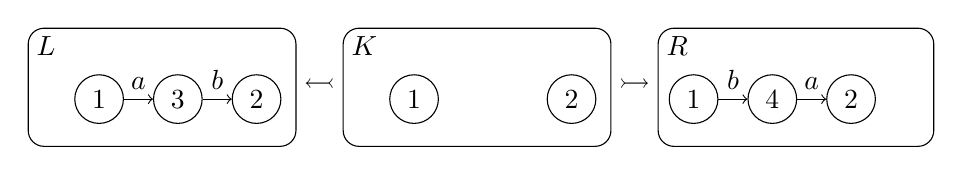
\begin{tikzpicture}[baseline=-3ex]
                    \graphbox{\( L \)}{0mm}{-3mm}{34mm}{15mm}{2mm}{2mm}{
                        \coordinate (o) at (0mm,-11mm); 
                        \node[draw,circle] (l1) at ($(o)+(-10mm,0mm)$) {1};
                        \node[draw,circle] (l2) at ($(l1)+(2,0)$) {2};
                        \node[draw,circle] (l3) at ($(l1)+(1,0)$) {3};
                        \draw[->] (l1) -- (l3) node[midway,above] {$a$};
                        \draw[->] (l3) -- (l2) node[midway,above] {$b$};
                    } 
            
                    \graphbox{\( K \)}{40mm}{-3mm}{34mm}{15mm}{2mm}{2mm}{
                        \coordinate (o) at (0mm,-11mm); 
                        \node[draw,circle] (l1) at ($(o)+(-10mm,0mm)$) {1};
                        \node[draw,circle] (l2) at ($(l1)+(2,0)$) {2};
                    }  
            
                    \graphbox{\( R \)}{80mm}{-3mm}{35mm}{15mm}{2mm}{2mm}{
                        \coordinate (o) at (-5mm,-11mm); 
                        \node[draw,circle] (l1) at ($(o)+(-10mm,0mm)$) {1};
                        % \node[draw,circle] (l2) at ($(l1)+(3,0)$) {2};
                        \node[draw,circle] (l3) at ($(l1)+(1,0)$) {4};
                        \node[draw,circle] (l4) at ($(l1)+(2,0)$) {2};
                        \draw[->] (l1) -- (l3) node[midway,above] {$b$};
                        \draw[->] (l3) -- (l4) node[midway,above] {$a$};
                        % \draw[->] (l4) -- (l2) node[midway,above] {$a$};
                    }    
                    \node () at (37mm,-10mm) {\( \leftarrowtail \)}; % K -> L
                    \node () at (77mm,-10mm) {\( \rightarrowtail \)}; % K -> R
                \end{tikzpicture}
                }
            % \end{center}  
 
\textcolor{blue}{Looping}:
        \begin{center}
            \resizebox{0.8\textwidth}{!}{
              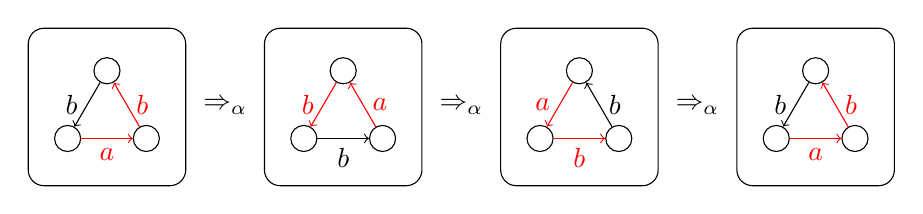
\begin{tikzpicture}
              \graphbox{\( \)}{0mm}{0mm}{20mm}{20mm}{-5mm}{-14mm}{
                  \node[draw,circle] (x) at (0,0) {};
                  \node[draw,circle] (y) at (1,0) {};
                  \node[draw,circle] (z) at (0.5,0.86) {};
                  \draw[->,red] (x) -- node[midway,below] {$a$} (y) ;
                  \draw[->,red] (y) -- node[midway,right] {$b$} (z) ;
                  \draw[->] (z) -- node[midway,left] {$b$} (x) ;
              } 
              \node () at (25mm,-10mm) {\( \Rightarrow_\alpha \)};
              \graphbox{\( \)}{30mm}{0mm}{20mm}{20mm}{-5mm}{-14mm}{
                  \node[draw,circle] (x) at (0,0) {};  
                  \node[draw,circle] (y) at (1,0) {};
                  \node[draw,circle] (z) at (0.5,0.86) {};
                  \draw[->] (x) -- node[midway,below] {$b$} (y) ;
                  \draw[->,red] (y) -- node[midway,right] {$a$} (z) ;
                  \draw[->,red] (z) -- node[midway,left] {$b$} (x) ;
              } 
              \node () at (55mm,-10mm) {\( \Rightarrow_\alpha \)};
              \graphbox{\( \)}{60mm}{0mm}{20mm}{20mm}{-5mm}{-14mm}{
                  \node[draw,circle] (x) at (0,0) {};  
                  \node[draw,circle] (y) at (1,0) {};
                  \node[draw,circle] (z) at (0.5,0.86) {};
                  \draw[->,red] (x) -- node[midway,below] {$b$} (y) ;
                  \draw[->] (y) -- node[midway,right] {$b$} (z) ;
                  \draw[->,red] (z) -- node[midway,left] {$a$} (x) ;
              }
              \node () at (85mm,-10mm) {\( \Rightarrow_\alpha \)};
              \graphbox{\( \)}{90mm}{0mm}{20mm}{20mm}{-5mm}{-14mm}{
                  \node[draw,circle] (x) at (0,0) {};   
                  \node[draw,circle] (y) at (1,0) {};
                  \node[draw,circle] (z) at (0.5,0.86) {};
                  \draw[->,red] (x) -- node[midway,below] {$a$} (y) ;
                  \draw[->,red] (y) -- node[midway,right] {$b$} (z) ;
                  \draw[->] (z) -- node[midway,left] {$b$} (x) ;
              }
          \end{tikzpicture}
          }
        \end{center}

     Rule $b$:
%   \begin{center}  
                \resizebox{0.85\textwidth}{!}{ 
                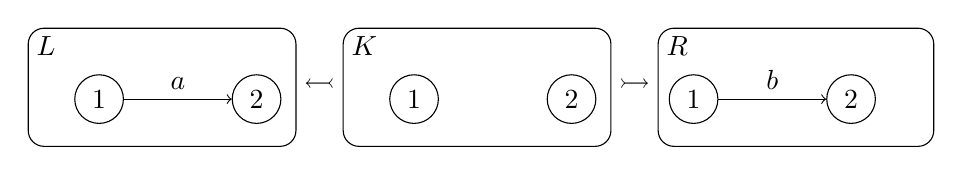
\begin{tikzpicture}[baseline=-3ex]
                    \graphbox{\( L \)}{0mm}{-3mm}{34mm}{15mm}{2mm}{2mm}{
                        \coordinate (o) at (0mm,-11mm); 
                        \node[draw,circle] (l1) at ($(o)+(-10mm,0mm)$) {1};
                        \node[draw,circle] (l2) at ($(l1)+(2,0)$) {2};
                        % \node[draw,circle] (l3) at ($(l1)+(1,0)$) {3};
                        \draw[->] (l1) -- (l2) node[midway,above] {$a$};
                    } 
            
                    \graphbox{\( K \)}{40mm}{-3mm}{34mm}{15mm}{2mm}{2mm}{
                        \coordinate (o) at (0mm,-11mm); 
                        \node[draw,circle] (l1) at ($(o)+(-10mm,0mm)$) {1};
                        \node[draw,circle] (l2) at ($(l1)+(2,0)$) {2};
                    }  
            
                    \graphbox{\( R \)}{80mm}{-3mm}{35mm}{15mm}{2mm}{2mm}{
                        \coordinate (o) at (-5mm,-11mm); 
                        \node[draw,circle] (l1) at ($(o)+(-10mm,0mm)$) {1};
                        % \node[draw,circle] (l2) at ($(l1)+(3,0)$) {2};
                         % \node[draw,circle] (l3) at ($(l1)+(1,0)$) {4};
                        \node[draw,circle] (l4) at ($(l1)+(2,0)$) {2};
                        \draw[->] (l1) -- (l4) node[midway,above] {$b$};
                        % \draw[->] (l4) -- (l2) node[midway,above] {$a$};
                    }    
                    \node () at (37mm,-10mm) {\( \leftarrowtail \)}; % K -> L
                    \node () at (77mm,-10mm) {\( \rightarrowtail \)}; % K -> R
                \end{tikzpicture}
                }
            % \end{center}  
  
\vspace{2mm}
\textcolor{blue}{Termination} by the number of edges labeled by \enquote{a}.

        \begin{center}
          \resizebox{0.4\textwidth}{!}{
              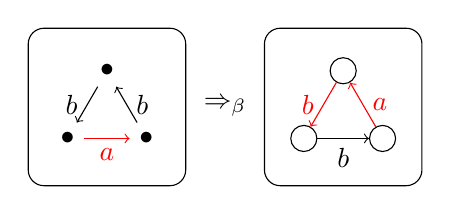
\begin{tikzpicture}
                \graphbox{\( \)}{0mm}{0mm}{20mm}{20mm}{-5mm}{-14mm}{
                  \node (x) at (0,0) {$\bullet$};  
                  \node (y) at (1,0) {$\bullet$};
                  \node (z) at (0.5,0.86) {$\bullet$};
                  \draw[->,red] (x) -- node[midway,below] {$a$} (y) ;
                  \draw[->] (y) -- node[midway,right] {$b$} (z) ;
                  \draw[->] (z) -- node[midway,left] {$b$} (x) ;
                } 
                \node () at (25mm,-10mm) {\( \Rightarrow_\beta \)};
                \graphbox{\( \)}{30mm}{0mm}{20mm}{20mm}{-5mm}{-14mm}{
                    \node[draw,circle] (x) at (0,0) {};  
                    \node[draw,circle] (y) at (1,0) {};
                    \node[draw,circle] (z) at (0.5,0.86) {};
                    \draw[->] (x) -- node[midway,below] {$b$} (y) ;
                    \draw[->,red] (y) -- node[midway,right] {$a$} (z) ;
                    \draw[->,red] (z) -- node[midway,left] {$b$} (x) ;
                }
            \end{tikzpicture}
          }
        \end{center}
\end{frame}

\section{Termination of Injective DPO Graph Rewriting using Morphism Counting}
\begin{frame}
  \tableofcontents[currentsection,hideothersubsections]
\end{frame}


\begin{frame}{Pre-graphs}
 Pre-graphs are graphs with missing nodes and dangling edges.
 
 Example:

        \begin{center}
            \resizebox{0.6\textwidth}{!}{
            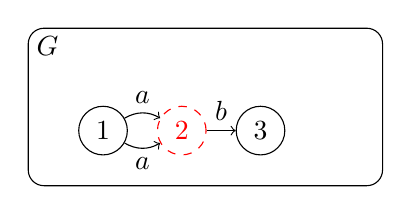
\begin{tikzpicture}
                \graphbox{\( G \)}{00mm}{-20mm}{45mm}{20mm}{2mm}{-5mm}{ 
                    \coordinate (o) at (-5mm,-8mm); 
                    \node[draw,circle] (l1) at ($(o)+(-10mm,0mm)$) {1};
                    % \node[draw,circle] (l2) at ($(l1)+(3,0)$) {};
                    \node[draw,circle,dashed,red] (l3) at ($(l1)+(1,0)$) {2};
                    \node[draw,circle] (l4) at ($(l1)+(2,0)$) {3};
                    \draw[->] (l1) edge[bend right]  node[midway,below] {$a$} (l3);
                    \draw[->] (l1) edge[bend left] node[midway,above] {$a$}  (l3);
                    \draw[->] (l3) -- (l4) node[midway,above] {$b$};
                    % \draw[->] (l4) -- (l2) node[midway,above] {$a$};
                }  
            \end{tikzpicture} 
        }
        \end{center} 

    The pregraph $G$ has 
    \begin{itemize}
      \item 2 existing nodes,
      \item 1 missing node,
      \item 3 dangling edges.
    \end{itemize}
\end{frame}

\begin{frame}{Pre-graph operations}
    \textcolor{red}{Union} of two pre-graphs $C \mathop{\subseteq} G$ and $R \mathop{\subseteq} G$, denoted $C \mathop{\cup} R$:
    % \vspace{1mm}
\begin{center}
    \resizebox{\textwidth}{!}{
        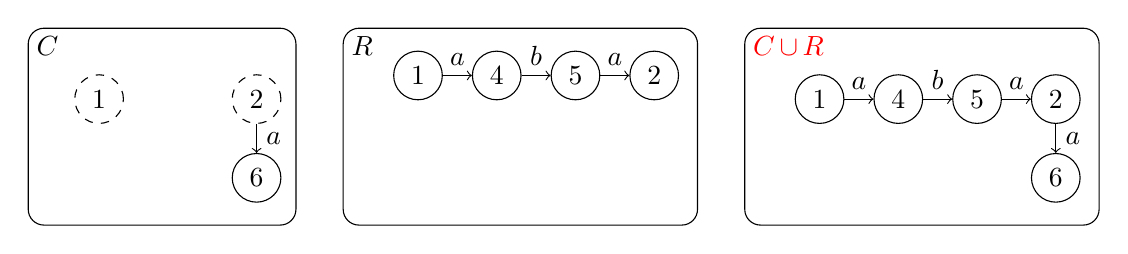
\begin{tikzpicture}          
            \graphbox{\( C  \)}{0mm}{-22mm}{34mm}{25mm}{2mm}{-3mm}{
                \coordinate (o) at (0mm,-6mm); 
                \node[draw,circle,dashed] (l1) at ($(o)+(-10mm,0mm)$) {1};
                \node[draw,circle,dashed] (l2) at ($(l1)+(2,0)$) {2};
                \node[draw,circle] (l4) at ($(l2)+(0,-1)$) {6};
                \draw[->] (l2) -- (l4) node[midway,right] {$a$};
                % \draw[->] (l2) edge[out=-135,in=-45]node[midway,below] {$a$} (l1) ;
                % \node[ draw,circle] (l6) at ($(l1)+(0,-1)$) {7};
                % \draw[<-] (l1) -- (l6) node[midway,left] {$a$};
            }    
            \graphbox{\( R \)}{40mm}{-22mm}{45mm}{25mm}{2mm}{2mm}{
                \coordinate (o) at (-5mm,-8mm); 
                \node[draw,circle] (l1) at ($(o)+(-10mm,0mm)$) {1};
                \node[draw,circle] (l2) at ($(l1)+(3,0)$) {2};
                \node[draw,circle] (l3) at ($(l1)+(1,0)$) {4};
                \node[draw,circle] (l4) at ($(l1)+(2,0)$) {5};
                \draw[->] (l1) -- (l3) node[midway,above] {$a$};
                \draw[->] (l3) -- (l4) node[midway,above] {$b$};
                \draw[->] (l4) -- (l2) node[midway,above] {$a$};
            } 
            \graphbox{\textcolor{red}{\(C \mathop{\cup} R \)}}{91mm}{-22mm}{45mm}{25mm}{2mm}{-3mm}{
                \coordinate (o) at (-5mm,-6mm); 
                \node[draw,circle] (l1) at ($(o)+(-10mm,0mm)$) {1};
                \node[draw,circle] (l2) at ($(l1)+(3,0)$) {2};
                \node[draw,circle] (l3) at ($(l1)+(1,0)$) {4};
                \node[draw,circle] (l4) at ($(l1)+(2,0)$) {5};
                \node[ draw,circle] (l5) at ($(l2)+(0,-1)$) {6};
                % \node[ draw,circle] (l6) at ($(l1)+(0,-1)$) {7};
                % \draw[<-] (l1) -- (l6) node[midway,left] {$a$};
                \draw[->] (l1) -- (l3) node[midway,above] {$a$};
                \draw[->] (l3) -- (l4) node[midway,above] {$b$};
                \draw[->] (l4) -- (l2) node[midway,above] {$a$};
                \draw[->] (l2) -- (l5) node[midway,right] {$a$};
                % \draw[->] (l2) edge[out=-135,in=-45]node[midway,below] {$a$} (l1) ;
            }    
             
        \end{tikzpicture}
    }
    \end{center}
\textcolor{red}{Relative complement} of $R$ in $H$ where $R \mathop{\subseteq} H$, denoted $H \mathop{\setminus} R$: 
    \begin{center}
  \resizebox{\textwidth}{!}{
        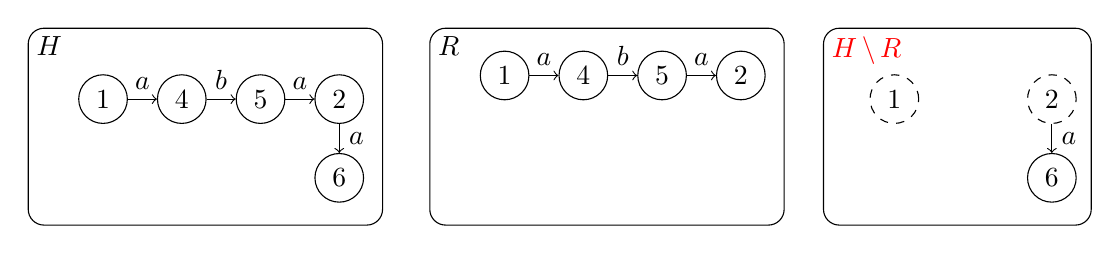
\begin{tikzpicture}       
            \graphbox{\( H \)}{-11mm}{-22mm}{45mm}{25mm}{2mm}{-3mm}{
                \coordinate (o) at (-5mm,-6mm); 
                \node[draw,circle] (l1) at ($(o)+(-10mm,0mm)$) {1};
                \node[draw,circle] (l2) at ($(l1)+(3,0)$) {2};
                \node[draw,circle] (l3) at ($(l1)+(1,0)$) {4};
                \node[draw,circle] (l4) at ($(l1)+(2,0)$) {5};
                \node[ draw,circle] (l5) at ($(l2)+(0,-1)$) {6};
                \draw[->] (l1) -- (l3) node[midway,above] {$a$};
                \draw[->] (l3) -- (l4) node[midway,above] {$b$};
                \draw[->] (l4) -- (l2) node[midway,above] {$a$};
                \draw[->] (l2) -- (l5) node[midway,right] {$a$};
                % \draw[->] (l2) edge[out=-135,in=-45]node[midway,below] {$a$} (l1) ;
            }  
            \graphbox{\( R \)}{40mm}{-22mm}{45mm}{25mm}{2mm}{2mm}{
                \coordinate (o) at (-5mm,-8mm); 
                \node[draw,circle] (l1) at ($(o)+(-10mm,0mm)$) {1};
                \node[draw,circle] (l2) at ($(l1)+(3,0)$) {2};
                \node[draw,circle] (l3) at ($(l1)+(1,0)$) {4};
                \node[draw,circle] (l4) at ($(l1)+(2,0)$) {5};
                \draw[->] (l1) -- (l3) node[midway,above] {$a$};
                \draw[->] (l3) -- (l4) node[midway,above] {$b$};
                \draw[->] (l4) -- (l2) node[midway,above] {$a$};
            }     
            \graphbox{\textcolor{red}{\( H \mathop{\setminus} R  \)}}{90mm}{-22mm}{34mm}{25mm}{2mm}{-3mm}{
                \coordinate (o) at (0mm,-6mm); 
                \node[draw,dashed,circle] (l1) at ($(o)+(-10mm,0mm)$) {1};
                \node[draw,dashed,circle] (l2) at ($(l1)+(2,0)$) {2};
                \node[draw,circle] (l4) at ($(l2)+(0,-1)$) {6};
                \draw[->] (l2) -- (l4) node[midway,right] {$a$};
                % \draw[->] (l2) edge[out=-135,in=-45]node[midway,below] {$a$} (l1) ;
            }   
        \end{tikzpicture}
    }
    \end{center}

    % Remark : \textcolor{red}{$H \mathop{\setminus} R$ is not always a graph.}
\end{frame}

\begin{frame}{test}
\end{frame}

\section{Etending the Type Graph Method to Non-well-founded Semirings}
\begin{frame}
  \tableofcontents[currentsection, hideothersubsections]
\end{frame}

% \begin{frame}{Plan}
%   \begin{itemize}
%     \item Type graph method with weights from well-founded semirings explained with an example
%     \item Observation
%     \item Extension : type graph method with weights from non-well-founded semirings
%     \item Complexity comparison
%     \item Experimental results and analysis
%     \item Conclusion
%   \end{itemize}
% \end{frame}


% \begin{frame}{Weighted Type Graph over Real Numbers}
%   \begin{itemize}
%     \item finite directed graph
%     \item edge-labeled
%     \item weights are positive real numbers
%     \item weights are superscripts
%   \end{itemize}
%       \begin{center}
%         \begin{tikzpicture}
%             \graphbox{}{0mm}{0mm}{32mm}{28mm}{-10mm}{-14mm}{
%                 \node[draw,circle] (1) at (0,0) {};
%                 \node[draw,circle] (2) at (2,0) {};
%                 \draw[->] (1) edge[loop above] node[midway, above] {$a^{1.0}$} (1) ;
%                 \draw[->] (1) edge[loop below] node[midway, below] {$b^{1.0}$} (1) ;
%                 \draw[->] (1) edge[bend left] node[midway, above] {$a^{1.0}$}  (2)  ;
%                 \draw[->] (2) edge[bend left] node[midway, below] {$a^{1.0}$} (1)   ;
%             }
%         \end{tikzpicture}
%     \end{center}
% \end{frame}

\begin{frame}{Graphs and Graph Morphisms}
\begin{adjustwidth}{-0.5cm}{0cm}
  \begin{itemize}
      \item \textbf{Graph morphisms}: structure-preserving mappings.
      % : function from graph $K$ to graph $L$ that preserves the structure of the graphs.
      \\
        Ex:
         \begin{center}
          \resizebox{0.8\textwidth}{!}{
          \begin{tikzpicture}
            \graphbox{\( G \)}{00mm}{-20mm}{45mm}{25mm}{2mm}{-10mm}{
                \coordinate (o) at (-5mm,-8mm); 
                \node[draw,circle] (l1) at ($(o)+(-10mm,0mm)$) {1};
                \node[draw,circle] (l2) at ($(l1)+(3,0)$) {2};
                \node[draw,circle] (l3) at ($(l1)+(1,0)$) {3};
                \node[draw,circle] (l4) at ($(l1)+(2,0)$) {4};
                \draw[->] (l1) -- (l3) node[midway,above] {$a$};
                \draw[->] (l3) -- (l4) node[midway,above] {$b$};
                \draw[->] (l4) -- (l2) node[midway,above] {$a$};
            }  
            \graphbox{\( H \)}{52mm}{-20mm}{50mm}{25mm}{2mm}{-10mm}{
                \coordinate (o) at (-5mm,-8mm); 
                \node[draw,circle] (l1) at ($(o)+(-1,0mm)$) {1};
                \node[draw,circle] (l2) at ($(l1)+(3,0)$) {2};
                \node[draw,circle] (l3) at ($(l1)+(1.5,0)$) {3\ 4};
                \draw[->] (l1) edge node[midway,above] {$a$} (l3);
                \draw[->] (l3) edge [loop above] node[midway,above] {$b$} (l3) ;
                \draw[->] (l3) -- (l2) node[midway,above] {$a$};
            }      
            \node () at (48mm,-30mm) {$\overset{h}{\rightarrow}$};
        \end{tikzpicture}
          }
         \end{center}
  \end{itemize} 
\end{adjustwidth}
\end{frame} 


\begin{frame}{Type graph method with weighted type graphs over natural numbers with an example}
  \begin{itemize}
    % \item 
% Natural Arithmetic Semiring: the usual arithmetic on natural numbers

    % \begin{itemize}
    %     \item $S$ : set 
    %     \item $\otimes$, $\mathop{\oplus}$ : binary operations on $S$
    %     \item $0$, $1$ : neutral elements for $\mathop{\oplus}$, $\otimes$
    %     \item $\prec$: a strict order 
    %     \item $\mathop{\preceq}$ : a reflexive order
    %     \item satisfies some conditions
    % \end{itemize}

    % Natural Arithmetic Semiring: $(\mathbb{N}, +, *, 0, 1, <, \leq)$ 
  \item Rule $\alpha$:
\begin{center} 
      \resizebox{0.9\textwidth}{!}{
      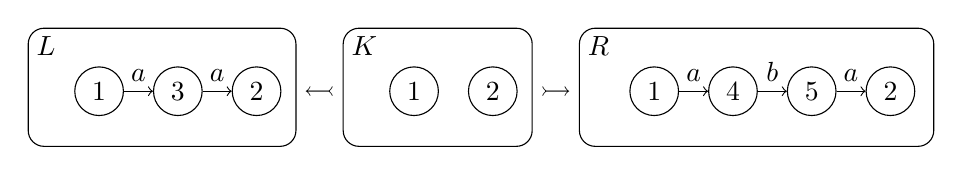
\begin{tikzpicture}
          \graphbox{$L$}{0mm}{0mm}{34mm}{15mm}{2mm}{-5mm}{
              \coordinate (o) at (0mm,-3mm); 
              \node[draw,circle] (l1) at ($(o)+(-10mm,0mm)$) {1};
              \node[draw,circle] (l2) at ($(l1)+(2,0)$) {2};
              \node[draw,circle] (l3) at ($(l1)+(1,0)$) {3};
              \draw[->] (l1) -- (l3) node[midway,above] {$a$};
              \draw[->] (l3) -- (l2) node[midway,above] {$a$};
          }     
          \graphbox{$K$}{40mm}{0mm}{24mm}{15mm}{2mm}{-5mm}{
              \coordinate (o) at (5mm,-3mm); 
              \node[draw,circle] (l1) at ($(o)+(-10mm,0mm)$) {1};
              \node[draw,circle] (l2) at ($(l1)+(1,0)$) {2};
              % \node[draw,circle] (l3) at ($(l1)+(1,0)$) {$\ $};
              % \draw[->] (l1) -- (l3) node[midway,above] {$a$};
              % \draw[->] (l3) -- (l2) node[midway,above] {$a$};
          }    
          \graphbox{$R$}{70mm}{0mm}{45mm}{15mm}{2mm}{-5mm}{
              \coordinate (o) at (-5mm,-3mm); 
              \node[draw,circle] (l1) at ($(o)+(-10mm,0mm)$) {1};
              \node[draw,circle] (l2) at ($(l1)+(3,0)$) {2};
              \node[draw,circle] (l3) at ($(l1)+(1,0)$) {4};
              \node[draw,circle] (l4) at ($(l1)+(2,0)$) {5};
              \draw[->] (l1) -- (l3) node[midway,above] {$a$};
              \draw[->] (l3) -- (l4) node[midway,above] {$b$};
              \draw[->] (l4) -- (l2) node[midway,above] {$a$};
          }    
          \node () at (37mm,-8mm) {$\leftarrowtail$};
          \node () at (67mm,-8mm) {$\rightarrowtail$};
          % \draw[>->] (51mm,2mm) -- (52mm,3mm);
      \end{tikzpicture}
      }
  \end{center}

    % Real Arithmetic Semiring $\mathcal{S} \mathop{=} (\mathbb{R}^+, +, *, 0, 1, <, \leq)$:
    % \begin{itemize}
    %   \item $\mathbb{R}^+$ : positive real numbers
    %   \item the usual addition $+$ and multiplication $*$
    %   \item the usual orders $<, \leq$
    % \end{itemize}

   \item Weighted type graph $T$ over
    % Natural Arithmetic Semiring:
    natural numbers:
    % \begin{itemize}
    %   \item finite directed graph
    %   \item edge-labeled
    %   \item weights are positive real numbers
    %   \item weights are superscripts
    % \end{itemize}
   \begin{center}
        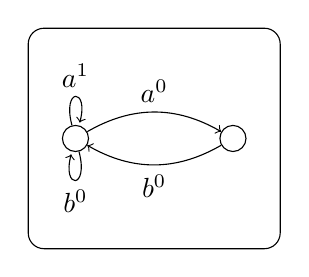
\begin{tikzpicture}
            \graphbox{}{0mm}{0mm}{32mm}{28mm}{-10mm}{-14mm}{
                \node[draw,circle] (1) at (0,0) {};
                \node[draw,circle] (2) at (2,0) {};
                \draw[->] (1) edge[loop above] node[midway, above] {$a^{1}$} (1) ;
                \draw[->] (1) edge[loop below] node[midway, below] {$b^{0}$} (1) ;
                \draw[->] (1) edge[bend left] node[midway, above] {$a^{0}$}  (2)  ;
                \draw[->] (2) edge[bend left] node[midway, below] {$b^{0}$} (1)   ;
            }
        \end{tikzpicture}
    \end{center}
  \end{itemize}
    % We are going to show 
    %   \begin{itemize}
    %     \item how to use $T$ to prove termination of $\alpha$, and
    %     \item the reduced complexity by using real numbers instead of integers.
    %   \end{itemize}
\end{frame}

\begin{frame}{Morphism Weight}

\begin{itemize}
  \item The weight of $h : L \mathop{\to} T$ is
  % Weight function $w : \opn{Edges}(T) \mathop{\to} \mathbb{N}$ 
  % The weight $ w_T(h) $ :  
%   is defined as:  
% $$
% w_T(h) \overset{def}{=} \prod_{e \mathop{\in} \opn{Edges}(L)} w(h(e)),
the sum of weights of all edges in $\opn{Im}(h)$.
   \item Example:
    
    \resizebox{0.8\textwidth}{!}{
        \begin{tikzpicture}
          \graphbox{\( L \)}{-50mm}{0mm}{40mm}{39mm}{2mm}{-6mm}{
            \coordinate (o) at (0mm,-10mm); 
            \node[draw,circle] (l1) at ($(o)+(-10mm,0mm)$) {1};
            \node[draw,circle] (l2) at ($(l1)+(2,0)$) {2};
            \node[draw,circle] (l3) at ($(l1)+(1,0)$) {3};
            \draw[red,->] (l1) -- (l3) node[midway,above] {$a$};
            \draw[red,->] (l3) -- (l2) node[midway,above] {$a$};
        } 
            \graphbox{$T$}{0mm}{0mm}{40mm}{39mm}{-10mm}{-17mm}{
                \node[draw,circle] (1) at (0,0) {$1\ 2$};
                \node[draw,circle] (2) at (2,0) {3};
                \draw[->] (1) edge[loop above] node[midway, above] {$a^{1}$} (1);
                \draw[->] (1) edge[loop below] node[midway, below] {$b^{0}$} (1);
                \draw[->,red] (1) edge[bend left] node[midway, above] {$a^{0}$}  (2);
                \draw[->,red] (2) edge[bend left] node[midway, below] {$b^{0}$} (1);
            }
            \node () at (-5mm,-15mm) {$\overset{h}{\to}$};
        \end{tikzpicture}
        }

        $ w_T(h) \mathop{=} 0 + 0 \mathop{=} 0$
\end{itemize}

 

   
\end{frame}
 

\begin{frame}{Graph Weight} 
  
 $w_T(L)$: the minimum weight $w_T(h)$ of all morphisms \( h : L \mathop{\to} T \)

Example : 

        \resizebox{0.3\textwidth}{!}{
              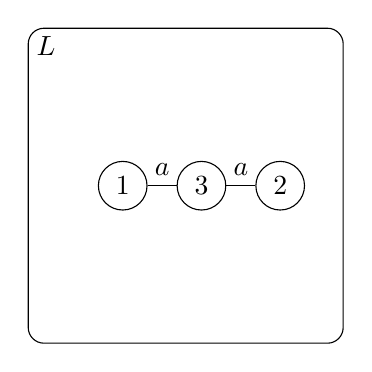
\begin{tikzpicture}
                            \graphbox{\(L\)}{-50mm}{0mm}{40mm}{40mm}{2mm}{-10mm}{
                            \coordinate (o) at (0mm,-10mm); 
                            \node[draw,circle] (l1) at ($(o)+(-10mm,0mm)$) {1};
                            \node[draw,circle] (l2) at ($(l1)+(2,0)$) {2};
                            \node[draw,circle] (l3) at ($(l1)+(1,0)$) {3};
                            \draw[] (l1) -- (l3) node[midway,above] {$a$};
                            \draw[] (l3) -- (l2) node[midway,above] {$a$};
                        } 
          \end{tikzpicture}
        }
      \resizebox{0.3\textwidth}{!}{
          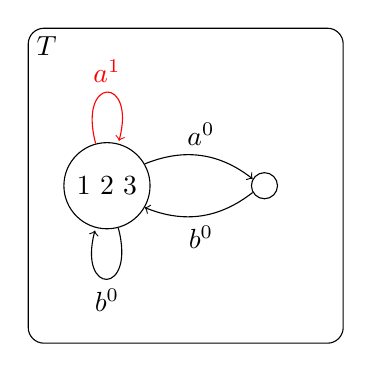
\begin{tikzpicture}
              \graphbox{$T$}{0mm}{0mm}{40mm}{40mm}{-10mm}{-20mm}{
                  \node[draw,circle] (1) at (0,0) {$1\ 2\ 3$};
                  \node[draw,circle] (2) at (2,0) {};
                  \draw[->,red] (1) edge[loop above] node[midway, above] {$a^{1}$} (1) ;
                  \draw[->] (1) edge[loop below] node[midway, below] {$b^{0}$} (1) ;
                  \draw[->] (1) edge[bend left] node[midway, above] {$a^{0}$}  (2)  ;
                  \draw[->] (2) edge[bend left] node[midway, below] {$b^{0}$} (1)   ;(1)   ;
              }
          \end{tikzpicture}
          }
        \resizebox{0.3\textwidth}{!}{
        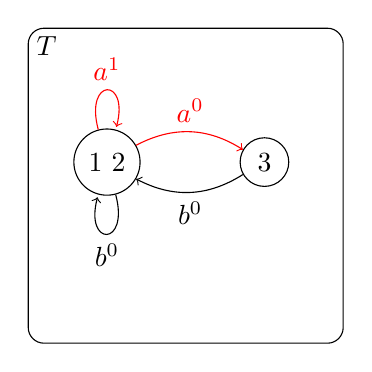
\begin{tikzpicture}
            \graphbox{$T$}{0mm}{0mm}{40mm}{40mm}{-10mm}{-17mm}{
                \node[draw,circle] (1) at (0,0) {$1\ 2$};
                \node[draw,circle] (2) at (2,0) {3};
                \draw[->,red] (1) edge[loop above] node[midway, above] {$a^{1}$} (1) ;
                \draw[->] (1) edge[loop below] node[midway, below] {$b^{0}$} (1) ;
                \draw[->,red] (1) edge[bend left] node[midway, above] {$a^{0}$}  (2)  ;
                \draw[->] (2) edge[bend left] node[midway, below] {$b^{0}$} (1)   ;
            }
        \end{tikzpicture}
        }
        $w_T(L) \mathop{=} \min \{1+1, 1+0\}\mathop{=} 1$       
\end{frame}

\begin{frame}
   \resizebox{0.3\textwidth}{!}{
        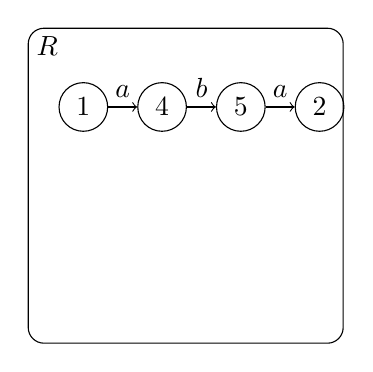
\begin{tikzpicture}
           \graphbox{$R$}{-50mm}{0mm}{40mm}{40mm}{2mm}{-10mm}{
              \coordinate (o) at (-5mm,0mm); 
              \node[draw,circle] (l1) at ($(o)+(-10mm,0mm)$) {1};
              \node[draw,circle] (l2) at ($(l1)+(3,0)$) {2};
              \node[draw,circle] (l3) at ($(l1)+(1,0)$) {4};
              \node[draw,circle] (l4) at ($(l1)+(2,0)$) {5};
              \draw[->] (l1) -- (l3) node[midway,above] {$a$};
              \draw[->] (l3) -- (l4) node[midway,above] {$b$};
              \draw[->] (l4) -- (l2) node[midway,above] {$a$};
          } 
        \end{tikzpicture}
        }
        \resizebox{0.3\textwidth}{!}{
            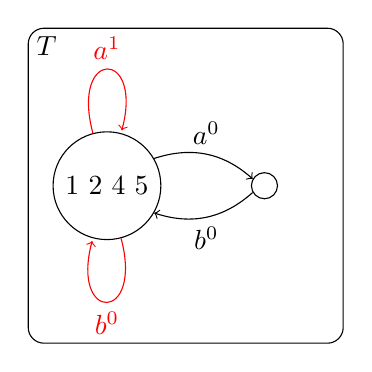
\begin{tikzpicture}
                \graphbox{$T$}{0mm}{0mm}{40mm}{40mm}{-10mm}{-20mm}{
                    \node[draw,circle] (1) at (0,0) {$1\ 2\ 4\ 5$};
                    \node[draw,circle] (2) at (2,0) {};
                    \draw[->,red] (1) edge[loop above] node[midway, above] {$a^{1}$} (1) ;
                    \draw[->,red] (1) edge[loop below] node[midway, below] {$b^{0}$} (1);
                    \draw[->] (1) edge[bend left] node[midway, above] {$a^{0}$}  (2);
                    \draw[->] (2) edge[bend left] node[midway, below] {$b^{0}$} (1);
                }
            \end{tikzpicture}
            }
        \resizebox{0.3\textwidth}{!}{
        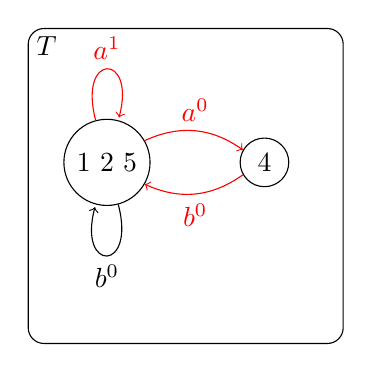
\begin{tikzpicture}
            \graphbox{$T$}{0mm}{0mm}{40mm}{40mm}{-10mm}{-17mm}{
                \node[draw,circle] (1) at (0,0) {$1\ 2\ 5$};
                \node[draw,circle] (2) at (2,0) {$4$};
                \draw[->,red] (1) edge[loop above] node[midway, above] {$a^{1}$} (1) ;
                \draw[->] (1) edge[loop below] node[midway, below] {$b^{0}$} (1) ;
                \draw[->,red] (1) edge[bend left] node[midway, above] {$a^{0}$}  (2)  ;
                \draw[->,red] (2) edge[bend left] node[midway, below] {$b^{0}$} (1);
            }
        \end{tikzpicture}
        }
        \resizebox{0.3\textwidth}{!}{
                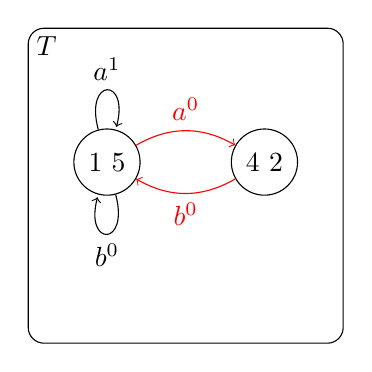
\begin{tikzpicture}
                    \graphbox{$T$}{0mm}{0mm}{40mm}{40mm}{-10mm}{-17mm}{
                        \node[draw,circle] (1) at (0,0) {$1\ 5$};
                        \node[draw,circle] (2) at (2,0) {$4\ 2$};
                        \draw[->] (1) edge[loop above] node[midway, above] {$a^{1}$} (1) ;
                        \draw[->] (1) edge[loop below] node[midway, below] {$b^{0}$} (1) ;
                        \draw[->,red] (1) edge[bend left] node[midway, above] {$a^{0}$}  (2)  ;
                        \draw[->,red] (2) edge[bend left] node[midway, below] {$b^{0}$} (1);
                    }
                \end{tikzpicture}
                }
      The weight of $R$ is $\min \{1+0+1, 0+0+1, 0 + 0 + 0\}\mathop{=} 0$
\end{frame}

\begin{frame}
  Since for all $G \mathop{\Rightarrow}_\alpha H$, we have $w_T(G) \mathop{\in} \mathbb{N}$, it remains to show that every rewriting step strictly decreases the weight.

  Not every weighted graph can be a weighted type graph
  It guarantees: for all $G \mathop{\Rightarrow}_\alpha H$, the weight of $G$ is defined and $w_T(G) \mathop{\in} \mathbb{N}$
\end{frame}

% \begin{frame}{Condition on Weighted Type Graph: for every rewriting step $G \mathop{\Rightarrow} H$, there exists a morphism $h : G \mathop{\to} T$.}
  

%   Consequence: for all $G \mathop{\Rightarrow} H$, $G$ has a weight and $w(G) \mathop{\geq} 0$.
%   % \begin{definition}
%   %   % Let $T \mathop{=} (T,\mathbb{E}, S, w)$ be a type graph, \(\rho \mathop{=} (L \xleftarrow{l} K \xrightarrow{r} R ) \) a DPO rewriting rule and $\mathfrak{F}$ a rewriting framework. 
%   %   A \textbf{context closure} for a rule $\rho$ and a $T$ is a morphism $c:L \mathop{\rightarrow} T$ such that for every possible DPO diagram depicted below,
%   %   there exists $\alpha : G \mathop{\rightarrow} T$ such that $m \mathop{\star} \alpha \mathop{=} c$.
%   %   \begin{center}
%   %       \begin{tikzpicture}[rotate=90]
%   %         \node (I) {$K$}; 
%   %         \node (L) [left of=I] {$L$};
%   %         \node (R) [right of=I] {$R$};
%   %         \node (G) [below of=L] {$G$};
%   %         \node (C) [below of=I] {$C$};
%   %         \node (H) [below of=R] {$H$};
%   %         \node (T) [left=of $(L)!0.5!(G)$] {$T$};
%   %         \draw [->] (L) to  node [label, above] {$c$}  (T);
%   %         \draw [->] (G) to  node [label, below] {$\alpha$} (T);
%   %         \draw [->] (I) to node [label, above] {$l$} (L);
%   %         \draw [->] (I) to node [label,above] {$r$} (R);
%   %         \draw [->] (L) to node [label, right] {$m$} (G);
%   %         \draw [->] (I) to (C);
%   %         \draw [->] (R) to (H);
%   %         \draw [->] (C) to (G);
%   %         \draw [->] (C) to (H);
%   %       \end{tikzpicture}
%   %     \end{center}
%   % \end{definition}
%   % Consequence:
% \end{frame}


% \begin{frame}{ 
%   every rewriting step strictly decreases the weight if:
%   % $w_T(G) \mathop{>} w_T(H)$ for every rewriting step $G \mathop{\Rightarrow}_\varphi H$ using rule $\varphi \mathop{=} L \xleftarrow{l} K \xrightarrow{r} R$ if
%   }
%   %  For $G \mathop{\Rightarrow} H$ defined by

%   %  \begin{center}
%   %     \resizebox{0.3\textwidth}{!}{
%   %       \begin{tikzpicture}
%   %           \node (I) at (0,0) {$K$};
%   %           \node (L) at (-2,0) {$L$};
%   %           \node (R) at (2,0) {$R$};
%   %           \node (G) at (-2,-2) {$G$};
%   %           \node (C) at (0,-2) {$C$};
%   %           \node (H) at (2,-2) {$H$};
%   %           \draw [->] (I) to  node [midway,below] {$l$} (L);
%   %           \draw [->] (I) to  node [midway,below] {$r$} (R);
%   %           \draw [->] (L) to node [midway,right] {$m$} (G);
%   %           \draw [->] (I) to node [midway,right] {$u$} (C);
%   %           \draw [->] (R) to node [midway,left] {$m'$} (H);
%   %           \draw [->] (C) to node [midway,above] {$l'$} (G);
%   %           \draw [->] (C) to node [midway,above] {$r'$} (H);
%   %           \node [at=($(I)!.5!(G)$)] {\normalfont PO};
%   %           \node [at=($(I)!.5!(H)$)] {\normalfont PO};
%   %         \end{tikzpicture}
%   %       }
%   % \end{center}
% % It suffices to show
% % \begin{theorem}
%   for every $t_K: K \mathop{\rightarrow} T$, 

% \begin{flalign*}
%   &\text{the sum of the weights of the morphisms $t_L$ that extend $t_K$} 
%   \\
%   &\mathop{\geq}
%   \\
%   &\text{the sum of the weights of the morphisms $t_R$ that extend $t_K$}
% \end{flalign*}

% %  $$ \sum ( w_T \{t_L :L \mathop{\to} T \mathop{\mid} \text{$t_L$ extends $t_K$}\} )
% %        -  \sum_{\substack{t_R: R \mathop{\rightarrow} T\\ t_K \mathop{=} t_R \circ r}}
% %             w_T(t_R) \mathop{\geq} 0 $$ 

% %     $$ \sum_{\substack{t_L: L \mathop{\rightarrow} T\\ t_K \mathop{=}  t_L \circ l }}
% %         w_T(t_L) -  \sum_{\substack{t_R: R \mathop{\rightarrow} T\\ t_K \mathop{=} t_R \circ r}}
% %             w_T(t_R) \mathop{\geq} 0 $$ 

% % for some $t_K: K \mathop{\rightarrow} T$,
% % $$ \sum_{\substack{t_L: L \mathop{\rightarrow} T\\ t_K \mathop{=} t_L \circ l}}
% %         w_T(t_L) - \sum_{\substack{t_R: R \mathop{\rightarrow} T\\ t_K \mathop{=} t_R \circ r}}
% %             w_T(t_R) \mathop{>} \delta $$ 
% for some $t_K: K \mathop{\rightarrow} T$,
% \begin{flalign*}
%   &\text{the sum of the weights of the morphisms $t_L$ that extend $t_K$} 
%   \\
%   &\mathop{>}
%   \\
%   &\text{the sum of the weights of the morphisms $t_R$ that extend $t_K$}
% \end{flalign*}
% % \end{theorem}   
% % then 
% %   \begin{center}
% %     $w_T(G) - w_T(H) \mathop{>} \delta$ for every rewriting step $G \mathop{\Rightarrow}_\varphi H$ using rule $\varphi$
% %   \end{center}
%   by \cite[Lemma 5.13]{endrullis2024generalized_arxiv_v2}.
%   % \resizebox{0.9\textwidth}{!}{
%   %   \begin{flalign*}
%   %     w_T(G) 
%   %         & \mathop{=} \sum_{t_K: K \mathop{\rightarrow} T} 
%   %         \left ( \sum_{\substack{t_C: C \mathop{\rightarrow} T\\ t_K \mathop{=} u \mathop{\star} t_C}}
%   %           w_T(t_C - u) \right ) 
%   %           \times
%   %         \left (\sum_{\substack{t_L: L \mathop{\rightarrow} T\\ t_K \mathop{=} t_L \circ l}}
%   %         w_T(t_L) \right )
%   %         \\
%   %     w_T(H) 
%   %         &  \mathop{\preceq} \sum_{t_K: K \mathop{\rightarrow} T} 
%   %         \left ( \sum_{\substack{t_C: C \mathop{\rightarrow} T\\ t_K \mathop{=} u \mathop{\star} t_C}}
%   %         w_T(t_C - u) \right ) 
%   %         \mathop{\times} 
%   %         \left ( \sum_{\substack{t_R: R \mathop{\rightarrow} T\\ t_K \mathop{=} t_R \circ r}}
%   %             w_T(t_R) \right ) \\
%   % \end{flalign*}
%   % }
% \end{frame}


\begin{frame}{Termination Condition}

  \begin{center} 
      \resizebox{0.9\textwidth}{!}{
      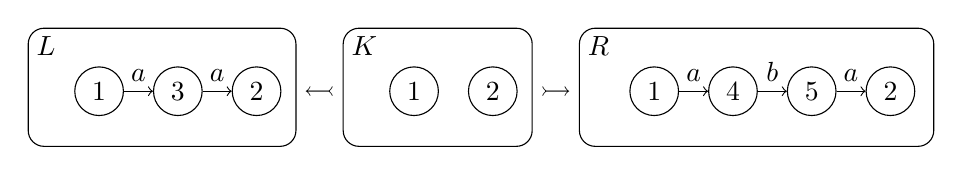
\begin{tikzpicture}
          \graphbox{$L$}{0mm}{0mm}{34mm}{15mm}{2mm}{-5mm}{
              \coordinate (o) at (0mm,-3mm); 
              \node[draw,circle] (l1) at ($(o)+(-10mm,0mm)$) {1};
              \node[draw,circle] (l2) at ($(l1)+(2,0)$) {2};
              \node[draw,circle] (l3) at ($(l1)+(1,0)$) {3};
              \draw[->] (l1) -- (l3) node[midway,above] {$a$};
              \draw[->] (l3) -- (l2) node[midway,above] {$a$};
          }     
          \graphbox{$K$}{40mm}{0mm}{24mm}{15mm}{2mm}{-5mm}{
              \coordinate (o) at (5mm,-3mm); 
              \node[draw,circle] (l1) at ($(o)+(-10mm,0mm)$) {1};
              \node[draw,circle] (l2) at ($(l1)+(1,0)$) {2};
              % \node[draw,circle] (l3) at ($(l1)+(1,0)$) {$\ $};
              % \draw[->] (l1) -- (l3) node[midway,above] {$a$};
              % \draw[->] (l3) -- (l2) node[midway,above] {$a$};
          }    
          \graphbox{$R$}{70mm}{0mm}{45mm}{15mm}{2mm}{-5mm}{
              \coordinate (o) at (-5mm,-3mm); 
              \node[draw,circle] (l1) at ($(o)+(-10mm,0mm)$) {1};
              \node[draw,circle] (l2) at ($(l1)+(3,0)$) {2};
              \node[draw,circle] (l3) at ($(l1)+(1,0)$) {4};
              \node[draw,circle] (l4) at ($(l1)+(2,0)$) {5};
              \draw[->] (l1) -- (l3) node[midway,above] {$a$};
              \draw[->] (l3) -- (l4) node[midway,above] {$b$};
              \draw[->] (l4) -- (l2) node[midway,above] {$a$};
          }    
          \node () at (37mm,-8mm) {$\leftarrowtail$};
          \node () at (67mm,-8mm) {$\rightarrowtail$};
          % \draw[>->] (51mm,2mm) -- (52mm,3mm);
      \end{tikzpicture}
      }
  \end{center}

  For every morphism $t_K: K \mathop{\rightarrow} T$, we define
\begin{itemize}
  \item $S(t_k,L)$ : the sum of the weights of the morphisms $t_L$ that extend $t_K$
  \item $S(t_k,R)$ : the sum of the weights of the morphisms $t_R$ that extend $t_K$
\end{itemize}
  
By \cite[Lemma 5.13]{endrullis2024generalized_arxiv_v2}, every rewriting step strictly decreases the weight if 
\begin{itemize}
  % \item for every $t_K: K \mathop{\rightarrow} T$, $$ S(t_K,L) \mathop{\geq} S(t_K,R) $$.
   \item for all $t_K: K \mathop{\rightarrow} T$,
  $$ S(t_K,L) \mathop{>} S(t_K,R) $$.
\end{itemize} 
% \end{theorem}   
% then 
%   \begin{center}
%     $w_T(G) - w_T(H) \mathop{>} \delta$ for every rewriting step $G \mathop{\Rightarrow}_\varphi H$ using rule $\varphi$
%   \end{center}

  % \resizebox{0.9\textwidth}{!}{
  %   \begin{flalign*}
  %     w_T(G) 
  %         & \mathop{=} \sum_{t_K: K \mathop{\rightarrow} T} 
  %         \left ( \sum_{\substack{t_C: C \mathop{\rightarrow} T\\ t_K \mathop{=} u \mathop{\star} t_C}}
  %           w_T(t_C - u) \right ) 
  %           \times
  %         \left (\sum_{\substack{t_L: L \mathop{\rightarrow} T\\ t_K \mathop{=} t_L \circ l}}
  %         w_T(t_L) \right )
  %         \\
  %     w_T(H) 
  %         &  \mathop{\preceq} \sum_{t_K: K \mathop{\rightarrow} T} 
  %         \left ( \sum_{\substack{t_C: C \mathop{\rightarrow} T\\ t_K \mathop{=} u \mathop{\star} t_C}}
  %         w_T(t_C - u) \right ) 
  %         \mathop{\times} 
  %         \left ( \sum_{\substack{t_R: R \mathop{\rightarrow} T\\ t_K \mathop{=} t_R \circ r}}
  %             w_T(t_R) \right ) \\
  % \end{flalign*}
  % }
\end{frame}

\begin{frame}{Example}
  There are $t_K^{11}, t_K^{12}, t_K^{21}, t_K^{22}:K \mathop{\rightarrow} T$ as depicted below:

    \begin{center}
        \resizebox{0.49\textwidth}{!}{
            \begin{tikzpicture}
            \graphbox{\( K \)}{-50mm}{0mm}{40mm}{30mm}{2mm}{-6mm}{
                \coordinate (o) at (0mm,-10mm); 
                \node[draw,circle] (l1) at ($(o)+(-10mm,0mm)$) {1};
                \node[draw,circle] (l2) at ($(l1)+(2,0)$) {2};
                % \node[draw,circle] (l3) at ($(l1)+(1,0)$) {3};
                % \draw[] (l1) -- (l3) node[midway,above] {$a$};
                % \draw[] (l3) -- (l2) node[midway,above] {$a$};
            } 
                \graphbox{$T$}{0mm}{0mm}{40mm}{30mm}{-10mm}{-15mm}{
                    \node[draw,circle] (1) at (0,0) {$1\ 2$};
                    \node[draw,circle] (2) at (2,0) {};
                    \draw[->] (1) edge[loop above] node[midway, above] {$a$} (1) ;
                    \draw[->] (1) edge[loop below] node[midway, below] {$b$} (1) ;
                    \draw[->] (1) edge[bend left] node[midway, above] {$a$}  (2)  ;
                    \draw[->] (2) edge[bend left] node[midway, below] {$a$} (1)   ;
                }
                \node () at (-5mm,-15mm) {$\overset{t_K^{11}}{\to}$};
            \end{tikzpicture}
            } 
            \resizebox{0.49\textwidth}{!}{
            \begin{tikzpicture}
                \graphbox{\( K \)}{-50mm}{0mm}{40mm}{30mm}{2mm}{-6mm}{
                \coordinate (o) at (0mm,-10mm); 
                \node[draw,circle] (l1) at ($(o)+(-10mm,0mm)$) {1};
                \node[draw,circle] (l2) at ($(l1)+(2,0)$) {2};
                % \node[draw,circle] (l3) at ($(l1)+(1,0)$) {3};
                % \draw[] (l1) -- (l3) node[midway,above] {$a$};
                % \draw[] (l3) -- (l2) node[midway,above] {$a$};
            } 
                \graphbox{$T$}{0mm}{0mm}{40mm}{30mm}{-10mm}{-15mm}{
                    \node[draw,circle] (1) at (0,0) {$1$};
                    \node[draw,circle] (2) at (2,0) {2};
                    \draw[->] (1) edge[loop above] node[midway, above] {$a$} (1) ;
                    \draw[->] (1) edge[loop below] node[midway, below] {$b$} (1) ;
                    \draw[->] (1) edge[bend left] node[midway, above] {$a$}  (2)  ; 
                    \draw[->] (2) edge[bend left] node[midway, below] {$a$} (1)   ;
                }
                \node () at (-5mm,-15mm) {$\overset{t_K^{12}}{\to}$};
            \end{tikzpicture}
            }
            \hspace{5mm}
            
            \resizebox{0.49\textwidth}{!}{
            \begin{tikzpicture}
                \graphbox{\( K \)}{-50mm}{0mm}{40mm}{30mm}{2mm}{-6mm}{
                \coordinate (o) at (0mm,-10mm); 
                \node[draw,circle] (l1) at ($(o)+(-10mm,0mm)$) {1};
                \node[draw,circle] (l2) at ($(l1)+(2,0)$) {2};
                % \node[draw,circle] (l3) at ($(l1)+(1,0)$) {3};
                % \draw[] (l1) -- (l3) node[midway,above] {$a$};
                % \draw[] (l3) -- (l2) node[midway,above] {$a$};
            } 
                \graphbox{$T$}{0mm}{0mm}{40mm}{30mm}{-10mm}{-15mm}{
                    \node[draw,circle] (1) at (0,0) {2};
                    \node[draw,circle] (2) at (2,0) {1};
                    \draw[->] (1) edge[loop above] node[midway, above] {$a$} (1) ;
                    \draw[->] (1) edge[loop below] node[midway, below] {$b$} (1) ;
                    \draw[->] (1) edge[bend left] node[midway, above] {$a$}  (2)  ;
                    \draw[->] (2) edge[bend left] node[midway, below] {$a$} (1)   ;
                }
                \node () at (-5mm,-15mm) {$\overset{t_K^{21}}{\to}$};
            \end{tikzpicture}
            }
            \resizebox{0.49\textwidth}{!}{
            \begin{tikzpicture}
                \graphbox{\( K \)}{-50mm}{0mm}{40mm}{30mm}{2mm}{-6mm}{
                \coordinate (o) at (0mm,-10mm); 
                \node[draw,circle] (l1) at ($(o)+(-10mm,0mm)$) {1};
                \node[draw,circle] (l2) at ($(l1)+(2,0)$) {2};
                % \node[draw,circle] (l3) at ($(l1)+(1,0)$) {3};
                % \draw[] (l1) -- (l3) node[midway,above] {$a$};
                % \draw[] (l3) -- (l2) node[midway,above] {$a$};
            } 
                \graphbox{$T$}{0mm}{0mm}{40mm}{30mm}{-10mm}{-15mm}{
                    \node[draw,circle] (1) at (0,0) {};
                    \node[draw,circle] (2) at (2,0) {$1\ 2$};
                    \draw[->] (1) edge[loop above] node[midway, above] {$a$} (1) ;
                    \draw[->] (1) edge[loop below] node[midway, below] {$b$} (1) ;
                    \draw[->] (1) edge[bend left] node[midway, above] {$a$}  (2)  ;
                    \draw[->] (2) edge[bend left] node[midway, below] {$a$} (1)   ;
                }
                \node () at (-5mm,-15mm) {$\overset{t_K^{22}}{\to}$};
            \end{tikzpicture}
            }
      \end{center}
\end{frame}   

\begin{frame}{Detail for $t_K^{11}$}
  \begin{center}
        \resizebox{0.49\textwidth}{!}{
        \begin{tikzpicture}
          \graphbox{\( L \)}{-50mm}{0mm}{40mm}{40mm}{2mm}{-6mm}{
            \coordinate (o) at (0mm,-10mm); 
            \node[draw,circle] (l1) at ($(o)+(-10mm,0mm)$) {1};
            \node[draw,circle] (l2) at ($(l1)+(2,0)$) {2};
            \node[draw,circle] (l3) at ($(l1)+(1,0)$) {3};
            \draw[] (l1) -- (l3) node[midway,above] {$a$};
            \draw[] (l3) -- (l2) node[midway,above] {$a$};
        } 
            \graphbox{$T$}{0mm}{0mm}{40mm}{40mm}{-10mm}{-17mm}{
                \node[draw,circle] (1) at (0,0) {$1\ 2$};
                \node[draw,circle] (2) at (2,0) {3};
                \draw[->] (1) edge[loop above] node[midway, above] {$a^{1}$} (1) ;
                \draw[->] (1) edge[loop below] node[midway, below] {$b^{1}$} (1) ;
                \draw[->,red] (1) edge[bend left] node[midway, above] {$a^{1}$}  (2)  ;
                \draw[->,red] (2) edge[bend left] node[midway, below] {$a^{1}$} (1)   ;
            }
            \node () at (-5mm,-15mm) {$\overset{h_{11}^1}{\to}$};
        \end{tikzpicture}
        }
        \resizebox{0.49\textwidth}{!}{
            \begin{tikzpicture}
              \graphbox{\(L\)}{-50mm}{0mm}{40mm}{40mm}{2mm}{-10mm}{
                \coordinate (o) at (0mm,-10mm); 
                \node[draw,circle] (l1) at ($(o)+(-10mm,0mm)$) {1};
                \node[draw,circle] (l2) at ($(l1)+(2,0)$) {2};
                \node[draw,circle] (l3) at ($(l1)+(1,0)$) {3};
                \draw[] (l1) -- (l3) node[midway,above] {$a$};
                \draw[] (l3) -- (l2) node[midway,above] {$a$};
            } 
                \graphbox{$T$}{0mm}{0mm}{40mm}{40mm}{-10mm}{-20mm}{
                    \node[draw,circle] (1) at (0,0) {$1\ 2\ 3$};
                    \node[draw,circle] (2) at (2,0) {};
                    \draw[->,red] (1) edge[loop above] node[midway, above] {$a^{1}$} (1) ;
                    \draw[->] (1) edge[loop below] node[midway, below] {$b^{1}$} (1) ;
                    \draw[->] (1) edge[bend left] node[midway, above] {$a^{1}$}  (2)  ;
                    \draw[->] (2) edge[bend left] node[midway, below] {$a^{1}$} (1)   ;(1)   ;
                }
                \node () at (-5mm,-15mm) {$\overset{h_{11}^2}{\to}$};
            \end{tikzpicture}
            }
      \end{center}
We have $S(t_k^{11},L) \mathop{=} w_\mathcal{T}(h_{11}^1)\mathop{+}w_\mathcal{T}(h_{11}^2)
        =(1 * 1)+(1 * 1)
        =2$

       \begin{center}
        \resizebox{0.49\textwidth}{!}{
        \begin{tikzpicture}
          \graphbox{\( R \)}{-55mm}{0mm}{45mm}{44mm}{1mm}{-22mm}{
            \coordinate (o) at (-5mm,-3mm); 
            \node[draw,circle] (l1) at ($(o)+(-10mm,0mm)$) {1};
            \node[draw,circle] (l2) at ($(l1)+(3,0)$) {2};
            \node[draw,circle] (l3) at ($(l1)+(1,0)$) {4};
            \node[draw,circle] (l4) at ($(l1)+(2,0)$) {5};
            \draw[->] (l1) -- (l3) node[midway,above] {$a$};
            \draw[->] (l3) -- (l4) node[midway,above] {$b$};
            \draw[->] (l4) -- (l2) node[midway,above] {$a$};
        } 
            \graphbox{$T$}{0mm}{0mm}{40mm}{44mm}{-10mm}{-22mm}{
                \node[draw,circle] (1) at (0,0) {$1\ 2\ 4\ 5$};
                \node[draw,circle] (2) at (2,0) {};
                \draw[->,red] (1) edge[loop above] node[midway, above] {$a^{1}$} (1) ;
                \draw[->,red] (1) edge[loop below] node[midway, below] {$b^{1}$} (1) ;
                \draw[->] (1) edge[bend left] node[midway, above] {$a^{1}$}  (2)  ;
                \draw[->] (2) edge[bend left] node[midway, below] {$a^{1}$} (1)   ;
            }
            \node () at (-5mm,-19mm) {$\overset{h_{11}^1}{\to}$};
        \end{tikzpicture}
        }
      \end{center}
    we have $S(t_k^{11},R) \mathop{=} w_\mathcal{T}(h_{11}^3) \mathop{=} 1 * 1 * 1  \mathop{=} 1$.

    Therefore, for $t_K^{11}$, we have: $S(t_k^{11},L) \mathop{=} 2 \mathop{>} 1 \mathop{=} S(t_k^{11},R)$.
\end{frame}

\begin{frame}{Example}
  There are $t_K^{11}, t_K^{12}, t_K^{21}, t_K^{22}:K \mathop{\rightarrow} T$ as depicted below:

    \begin{center}
        \resizebox{0.49\textwidth}{!}{
            \begin{tikzpicture}
            \graphbox{\( K \)}{-50mm}{0mm}{40mm}{30mm}{2mm}{-6mm}{
                \coordinate (o) at (0mm,-10mm); 
                \node[draw,circle] (l1) at ($(o)+(-10mm,0mm)$) {1};
                \node[draw,circle] (l2) at ($(l1)+(2,0)$) {2};
                % \node[draw,circle] (l3) at ($(l1)+(1,0)$) {3};
                % \draw[] (l1) -- (l3) node[midway,above] {$a$};
                % \draw[] (l3) -- (l2) node[midway,above] {$a$};
            } 
                \graphbox{$T$}{0mm}{0mm}{40mm}{30mm}{-10mm}{-15mm}{
                    \node[draw,circle] (1) at (0,0) {$1\ 2$};
                    \node[draw,circle] (2) at (2,0) {};
                    \draw[->] (1) edge[loop above] node[midway, above] {$a$} (1) ;
                    \draw[->] (1) edge[loop below] node[midway, below] {$b$} (1) ;
                    \draw[->] (1) edge[bend left] node[midway, above] {$a$}  (2)  ;
                    \draw[->] (2) edge[bend left] node[midway, below] {$a$} (1)   ;
                }
                \node () at (-5mm,-15mm) {$\overset{t_K^{11}}{\to}$};
            \end{tikzpicture}
            } 
            \resizebox{0.49\textwidth}{!}{
            \begin{tikzpicture}
                \graphbox{\( K \)}{-50mm}{0mm}{40mm}{30mm}{2mm}{-6mm}{
                \coordinate (o) at (0mm,-10mm); 
                \node[draw,circle] (l1) at ($(o)+(-10mm,0mm)$) {1};
                \node[draw,circle] (l2) at ($(l1)+(2,0)$) {2};
                % \node[draw,circle] (l3) at ($(l1)+(1,0)$) {3};
                % \draw[] (l1) -- (l3) node[midway,above] {$a$};
                % \draw[] (l3) -- (l2) node[midway,above] {$a$};
            } 
                \graphbox{$T$}{0mm}{0mm}{40mm}{30mm}{-10mm}{-15mm}{
                    \node[draw,circle] (1) at (0,0) {$1$};
                    \node[draw,circle] (2) at (2,0) {2};
                    \draw[->] (1) edge[loop above] node[midway, above] {$a$} (1) ;
                    \draw[->] (1) edge[loop below] node[midway, below] {$b$} (1) ;
                    \draw[->] (1) edge[bend left] node[midway, above] {$a$}  (2)  ;
                    \draw[->] (2) edge[bend left] node[midway, below] {$a$} (1)   ;
                }
                \node () at (-5mm,-15mm) {$\overset{t_K^{12}}{\to}$};
            \end{tikzpicture}
            }
            \hspace{5mm}
            
            \resizebox{0.49\textwidth}{!}{
            \begin{tikzpicture}
                \graphbox{\( K \)}{-50mm}{0mm}{40mm}{30mm}{2mm}{-6mm}{
                \coordinate (o) at (0mm,-10mm); 
                \node[draw,circle] (l1) at ($(o)+(-10mm,0mm)$) {1};
                \node[draw,circle] (l2) at ($(l1)+(2,0)$) {2};
                % \node[draw,circle] (l3) at ($(l1)+(1,0)$) {3};
                % \draw[] (l1) -- (l3) node[midway,above] {$a$};
                % \draw[] (l3) -- (l2) node[midway,above] {$a$};
            } 
                \graphbox{$T$}{0mm}{0mm}{40mm}{30mm}{-10mm}{-15mm}{
                    \node[draw,circle] (1) at (0,0) {2};
                    \node[draw,circle] (2) at (2,0) {1};
                    \draw[->] (1) edge[loop above] node[midway, above] {$a$} (1) ;
                    \draw[->] (1) edge[loop below] node[midway, below] {$b$} (1) ;
                    \draw[->] (1) edge[bend left] node[midway, above] {$a$}  (2)  ;
                    \draw[->] (2) edge[bend left] node[midway, below] {$a$} (1)   ;
                }
                \node () at (-5mm,-15mm) {$\overset{t_K^{21}}{\to}$};
            \end{tikzpicture}
            }
            \resizebox{0.49\textwidth}{!}{
            \begin{tikzpicture}
                \graphbox{\( K \)}{-50mm}{0mm}{40mm}{30mm}{2mm}{-6mm}{
                \coordinate (o) at (0mm,-10mm); 
                \node[draw,circle] (l1) at ($(o)+(-10mm,0mm)$) {1};
                \node[draw,circle] (l2) at ($(l1)+(2,0)$) {2};
                % \node[draw,circle] (l3) at ($(l1)+(1,0)$) {3};
                % \draw[] (l1) -- (l3) node[midway,above] {$a$};
                % \draw[] (l3) -- (l2) node[midway,above] {$a$};
            } 
                \graphbox{$T$}{0mm}{0mm}{40mm}{30mm}{-10mm}{-15mm}{
                    \node[draw,circle] (1) at (0,0) {};
                    \node[draw,circle] (2) at (2,0) {$1\ 2$};
                    \draw[->] (1) edge[loop above] node[midway, above] {$a$} (1) ;
                    \draw[->] (1) edge[loop below] node[midway, below] {$b$} (1) ;
                    \draw[->] (1) edge[bend left] node[midway, above] {$a$}  (2)  ;
                    \draw[->] (2) edge[bend left] node[midway, below] {$a$} (1)   ;
                }
                \node () at (-5mm,-15mm) {$\overset{t_K^{22}}{\to}$};
            \end{tikzpicture}
            }
      \end{center}
      \begin{itemize} 
        \item $t_K^{11}$ : $2 \mathop{>} 1$ 
        \item $t_K^{12}$ : $1 \mathop{\geq} 1$
        \item $t_K^{21}$ : $1 \mathop{\geq} 1$
        \item $t_K^{22}$ : $1 \mathop{\geq} 1$
      \end{itemize}
      Therefore, our Running Example is terminating by the weighted type graph $T$ over natural numbers.
\end{frame}  


\begin{frame}{Type Graph Method with Weighted Type Graphs over Well-founded Semirings}
  The \alert{existence} of suitable weighted type graphs is \alert{undecidable} in general.
\end{frame}



\begin{frame}{Searching for Weighted Type Graphs over Natural Numbers}
    User-specified parameters:
      \begin{itemize}
        \item $k$ nodes
        \item edge weights in $\{0, 1, \ldots, n\}$
      \end{itemize}   
    Assumption:
      \begin{itemize}
        \item no parallel edges of the same label 
      \end{itemize}
    The problem amounts to checking the satisfiability of an
existential Presburger arithmetic formula:
                \begin{itemize}
                  \item $k^2|\Sigma|$ binary variables
                  \item $k^2|\Sigma|$ integer variables
                \end{itemize} 
  Challenge:
  \begin{itemize}
    \item there are $2^{k^2|\Sigma|} \cdot n^{k^2|\Sigma|}$ possible assignments of weights
    \item $k$ and $n$ unknown à priori
  \end{itemize} 
\end{frame}

\begin{frame}{Solution: using real numbers instead of natural numbers.}
  
 Every rewriting step strictly decreases the weight if 
\begin{itemize}
  \item for every $t_K: K \mathop{\rightarrow} T$, 
  $$ S(t_K,L) \mathop{>} S(t_K,R) $$.
   \item there is $\delta > 0$ such that for some $t_K: K \mathop{\rightarrow} T$,
  $$ S(t_K,L) \mathop{>} S(t_K,R)\mathop{+}\delta$$.
\end{itemize} 
\end{frame}


\begin{frame}{Searching for Weighted Type Graphs over Real Numbers}
    User-specified parameters:
      \begin{itemize}
        \item $k$ nodes
        \item \crossout[red]{edge weights in $\{0, 1, \ldots, n\}$}
      \end{itemize}   
    Assumption:
      \begin{itemize}
        \item no parallel edges of the same label 
      \end{itemize}
    The problem amounts to checking the satisfiability of an
existential Presburger arithmetic formula:
                \begin{itemize}
                  \item $k^2|\Sigma|$ binary variables
                  \item $k^2|\Sigma|$ \textcolor{red}{real} variables
                \end{itemize} 
  Challenge:
  \begin{itemize}
    \item \crossout[red]{there are $2^{k^2|\Sigma|} \cdot n^{k^2|\Sigma|}$ possible assignments of weights}
    \item there are $2^{k^2|\Sigma|}$ linear programs which have polynomial-time average-case complexity
  \end{itemize} 
\end{frame}
 

% \begin{frame}{Concrete Semirings}
%   For each existing semiring over natural numbers (on the left), we propose a corresponding semiring over real numbers (on the right):

%   \begin{center}
%      Natural Tropical Semiring $\Leftrightarrow$ Real Tropical Semiring
%   \end{center}
%   \begin{center}
%      Natural Arctic Semiring $\Leftrightarrow$ Real Arctic Semiring
%   \end{center}
%   \begin{center}
%     Natural Arithmetic Semiring $\Leftrightarrow$ Real Arithmetic Semiring
%   \end{center}

%   Natural semirings: semirings on the left
 
%   Real semirings: semirings on the right
% \end{frame}

\begin{frame}{Implementation and Experimental Results}
  \alert{Implemented} in the tool LyonParallel
        \begin{itemize}
          % \item supports natural and real semirings
          \item supports natural and real numbers
          \item searches with natural and real numbers in parallel and cooperates between them
          % \item for edge-labeled directed graph rewriting
        \end{itemize}

  \alert{Tested} on examples from previous work:
  \begin{itemize}
    \item no need of user-specified upper bound on weights
    \item \alert{Acceleration} 
  \end{itemize}
\end{frame}

\section{Termination of Injective DPO Graph Rewriting using Morphism Counting with antipatterns}
\begin{frame}
  \tableofcontents[currentsection,hideothersubsections]
\end{frame}
\end{document} 